% Lammle, ch. 15
\chapter{Enhanced switched technologies}

Long ago, a company called Digital Equipment Corporation (DEC) created the
original version of \emph{Spanning Tree Protocol (STP)}. The IEEE later
created its own version of STP called 802.1d. Cisco has moved toward
another industry standard in its newer switches called 802.1w. We'll
explore both the old and new versions of STP in this chapter, but first,
I'll define some important STP basics.

Routing protocols like RIP, EIGRP, and OSPF have processes for
preventing loops from occurring at the network layer, but if you have
redundant physical links between your switches, these protocols won't do
a thing to stop loops from occurring at the data link layer.
That's exactly why STP was developed -- to put an end to loop issues in a layer~2 switched network.
It's also why we'll be thoroughly exploring the key features of this vital protocol as well as how it works within a
switched network in this chapter.

After covering STP in detail, we'll move on to explore EtherChannel.


\section{VLAN review}

As you may remember from ICND1, configuring VLANs is actually pretty
easy. It's just that figuring out which users you want in each VLAN is
not, and doing that can eat up a lot of your time! But once you've
decided on the number of VLANs you want to create and established which
users you want to belong to each one, it's time to bring your first VLAN
into the world.

To configure VLANs on a Cisco Catalyst switch, use the global config
\texttt{vlan} command. In the following example, I'm going to
demonstrate how to configure VLANs on the S1 switch by creating three
VLANs for three different departments -- again, remember that VLAN 1 is
the native and management VLAN by default:

\begin{cli}
S1(config)#vlan ?
  WORD        ISL VLAN IDs 1-4094
  access-map  Create vlan access-map or enter vlan access-map command mode
  dot1q       dot1q parameters
  filter      Apply a VLAN Map
  group       Create a vlan group
  internal    internal VLAN
S1(config)#vlan 2
S1(config-vlan)#name Sales
S1(config-vlan)#vlan 3
S1(config-vlan)#name Marketing
S1(config-vlan)#vlan 4
S1(config-vlan)#name Accounting
S1(config-vlan)#^Z
S1#
\end{cli}

In this output, you can see that you can create VLANs from 1 to 4094.
But this is only mostly true. As I said, VLANs can really only be
created up to 1001, and you can't use, change, rename, or delete VLANs 1
or 1002 through 1005 because they're reserved. The VLAN with numbers
above 1005 are called extended VLANs and won't be saved in the database
unless your switch is set to what is called VLAN Trunking Protocol (VTP)
transparent mode. You won't see these VLAN numbers used too often in
production. Here's an example of me attempting to set my S1 switch to
VLAN 4000 when my switch is set to VTP server mode (the default VTP
mode, which we'll talk about shortly):

\begin{cli}
S1#config t
S1(config)#vlan 4000
S1(config-vlan)#^Z
% Failed to create VLANs 4000
Extended VLAN(s) not allowed in current VTP mode.
%Failed to commit extended VLAN(s) changes.
\end{cli}

After you create the VLANs that you want, you can use the
\texttt{show\ vlan} command to check them out.
But notice that, by default, all ports on the switch are in VLAN 1.
To change the VLAN associated with a port, you need to go to each interface and specifically tell it which VLAN to be a part of.

\begin{center}\rule{0.5\linewidth}{0.5pt}\end{center}

%\includegraphics{images/note.png}
Remember that a created VLAN is unused
until it is assigned to a switch port or ports and that all ports are
always assigned in VLAN 1 unless set otherwise.

\begin{center}\rule{0.5\linewidth}{0.5pt}\end{center}

Once the VLANs are created, verify your configuration with the
\texttt{show\ vlan} command (\texttt{sh\ vlan} for short):

\begin{cli}
S1#sh vlan

VLAN Name               Status    Ports
---- ------------------ --------- -------------------------------
1    default            active    Fa0/1, Fa0/2, Fa0/3, Fa0/4
                                  Fa0/5, Fa0/6, Fa0/7, Fa0/8
                                  Fa0/9, Fa0/10, Fa0/11, Fa0/12
                                  Fa0/13, Fa0/14, Fa0/19, Fa0/20
                                  Fa0/21, Fa0/22, Fa0/23, Gi0/1
                                  Gi0/2
2    Sales              active
3    Marketing          active
4    Accounting         active
[output cut]
\end{cli}

If you want to see which ports are assigned to a particular VLAN (for
example, VLAN 200), you can obviously use the \texttt{show\ vlan}
command as shown above, or you can use the \texttt{show\ vlan\ id\ 200}
command to get ports assigned only to VLAN 200.

This may seem repetitive, but it's important, and I want you to remember
it: You can't change, delete, or rename VLAN 1 because it's the default
VLAN and you just can't change that -- period. It's also the native VLAN
of all switches by default, and Cisco recommends that you use it as your
management VLAN. If you're worried about security issues, then change
the native VLAN! Basically, any ports that aren't specifically assigned
to a different VLAN will be sent down to the native VLAN -- VLAN 1.

In the preceding S1 output, you can see that ports Fa0/1 through Fa0/14,
Fa0/19 through 23, and the Gi0/1 and Gi02 uplinks are all in VLAN 1. But
where are ports 15 through 18? First, understand that the
command\texttt{show\ vlan} only displays access ports, so now that you
know what you're looking at with the \texttt{show\ vlan} command, where
do you think ports Fa15--18 are? That's right! They are trunked ports.
Cisco switches run a proprietary protocol called \emph{Dynamic Trunk
Protocol (DTP)}, and if there is a compatible switch connected, they
will start trunking automatically, which is precisely where my four
ports are. You have to use the\texttt{show\ interfaces\ trunk} command
to see your trunked ports like this:

\begin{cli}
S1# show interfaces trunk
Port        Mode             Encapsulation  Status        Native vlan
Fa0/15      desirable        n-isl          trunking      1
Fa0/16      desirable        n-isl          trunking      1
Fa0/17      desirable        n-isl          trunking      1
Fa0/18      desirable        n-isl          trunking      1
 
Port        Vlans allowed on trunk
Fa0/15      1-4094
Fa0/16      1-4094
Fa0/17      1-4094
Fa0/18      1-4094
 
[output cut]
\end{cli}

This output reveals that the VLANs from 1 to 4094 are allowed across the trunk by default.
Another helpful command, which is also part of the Cisco exam
objectives, is the \texttt{show\ interfaces}
\texttt{interface}\texttt{\ switchport} command:

\begin{verbatim}
S1#sh interfaces fastEthernet 0/15 switchport
Name: Fa0/15
Switchport: Enabled
Administrative Mode: dynamic desirable
Operational Mode: trunk
Administrative Trunking Encapsulation: negotiate
Operational Trunking Encapsulation: isl
Negotiation of Trunking: On
Access Mode VLAN: 1 (default)
Trunking Native Mode VLAN: 1 (default)
Administrative Native VLAN tagging: enabled
Voice VLAN: none
[output cut]
\end{verbatim}

The highlighted output shows us the administrative mode of
\texttt{dynamic\ desirable}, that the port is a trunk port, and that DTP
was used to negotiate the frame-tagging method of ISL. It also
predictably shows that the native VLAN is the default of 1.

Now that we can see the VLANs created, we can assign switch ports to
specific ones. Each port can be part of only one VLAN, with the
exception of voice access ports. Using trunking, you can make a port
available to traffic from all VLANs. I'll cover that next.

\subsection{Assigning switch ports to VLANs}

You configure a port to belong to a VLAN by assigning a membership mode
that specifies the kind of traffic the port carries plus the number of
VLANs it can belong to. You can also configure each port on a switch to
be in a specific VLAN (access port) by using the
\texttt{inter}\texttt{face} \texttt{switchport} command. You can even
configure multiple ports at the same time with the
\texttt{interface\ range} command.

In the next example, I'll configure interface Fa0/3 to VLAN 3. This is
the connection from the S3 switch to the host device:

\begin{verbatim}
S3#config t
S3(config)#int fa0/3
S3(config-if)#switchport ?
  access         Set access mode characteristics of the interface
  autostate      Include or exclude this port from vlan link up calculation
  backup         Set backup for the interface
  block          Disable forwarding of unknown uni/multi cast addresses
  host           Set port host
  mode           Set trunking mode of the interface
  nonegotiate    Device will not engage in negotiation protocol on this
                 interface
  port-security  Security related command
  priority       Set appliance 802.1p priority
  private-vlan   Set the private VLAN configuration
  protected      Configure an interface to be a protected port
  trunk          Set trunking characteristics of the interface
  voice          Voice appliance attributes  voice
\end{verbatim}

Well now, what do we have here? There's some new stuff showing up in our
output now. We can see various commands -- some that I've already
covered, but no worries because I'm going to cover the \texttt{access},
\texttt{mode}, \texttt{nonegotiate}, and \texttt{trunk} commands very
soon. Let's start with setting an access port on S1, which is probably
the most widely used type of port you'll find on production switches
that have VLANs configured:

\begin{verbatim}
S3(config-if)#switchport mode ?
    access        Set trunking mode to ACCESS unconditionally
  dot1q-tunnel  set trunking mode to TUNNEL unconditionally
  dynamic       Set trunking mode to dynamically negotiate access or trunk mode
  private-vlan  Set private-vlan mode
  trunk         Set trunking mode to TRUNK unconditionally
 
S3(config-if)#switchport mode access
S3(config-if)#switchport access vlan 3
\end{verbatim}

By starting with the \texttt{switchport\ mode\ access} command, you're
telling the switch that this is a nontrunking layer~2 port. You can then
assign a VLAN to the port with the \texttt{switchport\ access} command.
Remember, you can choose many ports to configure simultaneously with the
\texttt{interface\ range} command.

Let's take a look at our VLANs now:

\begin{verbatim}
S3#show vlan
VLAN Name                       Status    Ports
---- ------------------------ --------- -------------------------------
1    default                   active     Fa0/4, Fa0/5, Fa0/6, Fa0/7
                                          Fa0/8, Fa0/9, Fa0/10, Fa0/11,
                                          Fa0/12, Fa0/13, Fa0/14, Fa0/19,
                                          Fa0/20, Fa0/21, Fa0/22, Fa0/23,
                                          Gi0/1,Gi0/2
 
2    Sales                     active
3    Marketing                 active    Fa0/3
\end{verbatim}

Notice that port Fa0/3 is now a member of VLAN 3. But, can you tell me where ports 1 and
2 are? And why aren't they showing up in the output of
\texttt{show\ vlan}? That's right, because they are trunk ports!

We can also see this with the
\texttt{show\ interfaces\ interface\ switchport} command:

\begin{verbatim}
S3#sh int fa0/3 switchport
Name: Fa0/3
Switchport: Enabled
Administrative Mode: static access
Operational Mode: static access
Administrative Trunking Encapsulation: negotiate
Negotiation of Trunking: Off
Access Mode VLAN: 3 (Marketing)
\end{verbatim}

The highlighted output shows that Fa0/3 is an access port and a member
of VLAN 3 (Marketing).

Before we move onto trunking and VTP, let's add a voice VLAN on our
switch. When an IP phone is connected to a switch port, this port should
have a voice VLAN associated with it. By creating a separate VLAN for
voice traffic, which of course you would do, what happens when you have
a PC or laptop that connects via Ethernet into an IP phone? The phone
connects to the Ethernet port and into one port on the switch. You're
now sending both voice and data to the single switch port.

All you need to do is add another VLAN to the same switch port like so
to fix this issue and separate the data at the switch port into two
VLANs:

\begin{verbatim}
S1(config)#vlan 10
S1(config-vlan)#name Voice
S1(config-vlan)#int g0/1
S1(config-if)#switchport voice vlan 10
\end{verbatim}

That's it. Well, sort of. If you plugged devices into each VLAN port,
they can only talk to other devices in the same VLAN. But as soon as you
learn a bit more about trunking, we're going to enable inter-VLAN
communication!

\subsection{Configuring trunk ports}

The 2960 switch only runs the IEEE 802.1q encapsulation method. To
configure trunking on a FastEthernet port, use the interface command
\texttt{switchport\ mode\ trunk}. It's a tad different on the 3560
switch.

The following switch output shows the trunk configuration on interfaces
Fa0/15--18 as set to \texttt{trunk}:

\begin{verbatim}
S1(config)#int range f0/15-18
S1(config-if-range)#switchport trunk encapsulation dot1q
S1(config-if-range)#switchport mode trunk
\end{verbatim}

If you have a switch that only runs the 802.1q encapsulation method, then you wouldn't use
the encapsulation command as I did in the preceding output. Let's check
out our trunk ports now:

\begin{verbatim}
S1(config-if-range)#do sh int f0/15 switchport
Name: Fa0/15
Switchport: Enabled
Administrative Mode: trunk
Operational Mode: trunk
Administrative Trunking Encapsulation: dot1q
Operational Trunking Encapsulation: dot1q
Negotiation of Trunking: On
Access Mode VLAN: 1 (default)
Trunking Native Mode VLAN: 1 (default)
Administrative Native VLAN tagging: enabled
Voice VLAN: none
\end{verbatim}

Notice that port Fa0/15 is a trunk and running 802.1q.
Let's take another look:

\begin{verbatim}
S1(config-if-range)#do sh int trunk
Port        Mode             Encapsulation  Status        Native vlan
Fa0/15      on               802.1q         trunking      1
Fa0/16      on               802.1q         trunking      1
Fa0/17      on               802.1q         trunking      1
Fa0/18      on               802.1q         trunking      1
Port        Vlans allowed on trunk
Fa0/15      1-4094
Fa0/16      1-4094
Fa0/17      1-4094
Fa0/18      1-4094
\end{verbatim}

Take note of the fact that ports 15--18 are now in the trunk mode of on
and the encapsulation is now 802.1q instead of the negotiated ISL.
Here's a description of the different options available when configuring
a switch interface:

\texttt{switchport\ mode\ access} I discussed this in the previous
section, but this puts the interface (access port) into permanent
nontrunking mode and negotiates to convert the link into a nontrunk
link. The interface becomes a nontrunk interface regardless of whether
the neighboring interface is a trunk interface. The port would be a
dedicated layer~2 access port.

\texttt{switchport\ mode\ dynamic\ auto} This mode makes the interface
able to convert the link to a trunk link. The interface becomes a trunk
interface if the neighboring
interface is set to
trunk or desirable mode. The default is \texttt{dynamic\ auto} on a lot
of Cisco switches, but that default trunk method is changing to
\texttt{dynamic\ desirable} on most new models.

\texttt{switchport\ mode\ dynamic\ desirable} This one makes the
interface actively attempt to convert the link to a trunk link. The
interface becomes a trunk interface if the neighboring interface is set
to \texttt{trunk}, \texttt{desirable}, or \texttt{auto} mode. This is
now the default switch port mode for all Ethernet interfaces on all new
Cisco switches.

\texttt{switchport\ mode\ trunk} Puts the interface into permanent
trunking mode and negotiates to convert the neighboring link into a
trunk link. The interface becomes a trunk interface even if the
neighboring interface isn't a trunk interface.

\texttt{switchport\ nonegotiate} Prevents the interface from generating
DTP frames. You can use this command only when the interface switchport
mode is access or trunk. You must manually configure the neighboring
interface as a trunk interface to establish a trunk link.

\begin{center}\rule{0.5\linewidth}{0.5pt}\end{center}

%\includegraphics{images/note.png}
Dynamic Trunking Protocol (DTP) is used
for negotiating trunking on a link between two devices as well as
negotiating the encapsulation type of either 802.1q or ISL. I use the
\texttt{nonegotiate} command when I want dedicated trunk ports; no
questions asked.

\begin{center}\rule{0.5\linewidth}{0.5pt}\end{center}

To disable trunking on an interface, use the
\texttt{switchport\ mode\ access} command, which sets the port back to a
dedicated layer~2 access switch port.

\paragraph{Defining the Allowed VLANs on a Trunk}

As I've mentioned, trunk ports send and receive information from all
VLANs by default, and if a frame is untagged, it's sent to the
management VLAN. Understand that this applies to the extended range
VLANs too.

But we can remove VLANs from the allowed list to prevent traffic from
certain VLANs from traversing a trunked link. I'll show you how you'd do
that, but first let me again demonstrate that all VLANs are allowed
across the trunk link by default:

\begin{verbatim}
S1# show interfaces trunk
[output cut]
Port        Vlans allowed on trunk
Fa0/15      1-4094
Fa0/16      1-4094
Fa0/17      1-4094
Fa0/18      1-4094
S1(config)#int f0/15
S1(config-if)#switchport trunk allowed vlan 4,6,12,15
S1(config-if)#do show int trunk
[output cut]
Port        Vlans allowed on trunk
Fa0/15      4,6,12,15
Fa0/16      1-4094
Fa0/17      1-4094
Fa0/18      1-4094
\end{verbatim}

The preceding command
affected the trunk link configured on S1 port Fa0/15, causing it to
permit all traffic sent and received for VLANs 4, 6, 12, and 15. You can
try to remove VLAN 1 on a trunk link, but it will still send and receive
management data like CDP, DTP, and VTP, so what's the point?

To remove a range of VLANs, just use the hyphen:

\begin{verbatim}
S1(config-if)#switchport trunk allowed vlan remove 4-8
\end{verbatim}

If by chance someone has removed some VLANs from a trunk link and you
want to set the trunk back to default, just use this command:

\begin{verbatim}
S1(config-if)#switchport trunk allowed vlan all
\end{verbatim}

Next, I want to show you how to configure a native VLAN for a trunk
before we start routing between VLANs.

\paragraph{Changing or Modifying the Trunk Native VLAN}

You can change the trunk port native VLAN from VLAN 1, which many people
do for security reasons. To change the native VLAN, use the following
command:

\begin{verbatim}
S1(config)#int f0/15
S1(config-if)#switchport trunk native vlan ?
  <1-4094>  VLAN ID of the native VLAN when this port is in trunking mode
\end{verbatim}

\begin{verbatim}
S1(config-if)#switchport trunk native vlan 4
1w6d: %CDP-4-NATIVE_VLAN_MISMATCH: Native VLAN mismatch discovered on FastEthernet0/15 (4), with S3 FastEthernet0/1 (1).
\end{verbatim}

So we've changed our native VLAN on our trunk link to 4, and by using
the \texttt{show\ running-config} command, I can see the configuration
under the trunk link:

\begin{verbatim}
S1#sh run int f0/15
Building configuration...
 
Current configuration : 202 bytes
!
interface FastEthernet0/15
 description 1st connection to S3
 switchport trunk encapsulation dot1q
 switchport trunk native vlan 4
 switchport trunk allowed vlan 4,6,12,15
 switchport mode trunk
end
 
S1#!
\end{verbatim}

Oops -- wait a minute!
You didn't think it would be this easy and would just start working, did
you? Of course not! Here's the rub: If all switches don't have the same
native VLAN configured on the given trunk links, then we'll start to
receive this error, which happened immediately after I entered the
command:

\begin{verbatim}
1w6d: %CDP-4-NATIVE_VLAN_MISMATCH: Native VLAN mismatch discovered
on FastEthernet0/15 (4), with S3 FastEthernet0/1 (1).
\end{verbatim}

Actually, this is a good, noncryptic error, so either we can go to the
other end of our trunk link(s) and change the native VLAN or we set the
native VLAN back to the default to fix it. Here's how we'd do that:

\begin{verbatim}
S1(config-if)#no switchport trunk native vlan
1w6d: %SPANTREE-2-UNBLOCK_CONSIST_PORT: Unblocking FastEthernet0/15
on VLAN0004. Port consistency restored.
\end{verbatim}

Now our trunk link is using the default VLAN 1 as the native VLAN.
Just remember that all switches on a given trunk must use the same native VLAN or you'll have some serious management problems.
These issues won't affect user data, just management traffic between switches.
Now, let's mix it up by connecting a router into our switched network and configure inter-VLAN communication.




\section{VLAN trunking protocol (VTP)}

Cisco created this one too. The basic goals of \emph{VLAN Trunking
Protocol (VTP)} are to manage all configured VLANs across a switched
internetwork and to maintain consistency throughout that network. VTP
allows you to add, delete, and rename VLANs -- information that is then
propagated to all other switches in the VTP domain.

Here's a list of some of the cool features VTP has to offer:

\begin{enumerate}
\tightlist
\item
  Consistent VLAN configuration across all switches in the network
\item
  VLAN trunking over mixed networks, such as Ethernet to ATM LANE or
  even FDDI
\item
  Accurate tracking and monitoring of VLANs
\item
  Dynamic reporting of added VLANs to all switches in the VTP domain
\item
  Adding VLANs using Plug and Play
\end{enumerate}

Very nice, but before you can get VTP to manage your VLANs across the
network, you have to create a VTP server (really, you don't need to even
do that since all switches default to VTP server mode, but just make
sure you have a server). All servers that need to share VLAN information
must use the same domain name, and a switch can be in only one domain at
a time. So basically, this means that a switch can share VTP domain
information with other switches only if they're configured into the same
VTP domain. You can use a VTP domain if you have more than one switch
connected in a network, but if you've got
all your switches in
only one VLAN, you just don't need to use VTP. Do keep in mind that VTP
information is sent between switches only via a trunk port.

Switches advertise VTP management domain information as well as a
configuration revision number and all known VLANs with any specific
parameters. But there's also something called \emph{VTP transparent
mode}. In it, you can configure switches to forward VTP information
through trunk ports but not to accept information updates or update
their VLAN databases.

If you've got sneaky users adding switches to your VTP domain behind
your back, you can include passwords, but don't forget -- every switch
must be set up with the same password. And as you can imagine, this
little snag can be a real hassle administratively!

Switches detect any added VLANs within a VTP advertisement and then
prepare to send information on their trunk ports with the newly defined
VLAN in tow. Updates are sent out as revision numbers that consist of
summary advertisements. Anytime a switch sees a higher revision number,
it knows the information it's getting is more current, so it will
overwrite the existing VLAN database with the latest information.

You should know these four requirements for VTP to communicate VLAN
information between switches:

\begin{enumerate}
\tightlist
\item
  The VTP version must be set the same
\item
  The VTP management domain name of both switches must be set the same.
\item
  One of the switches has to be configured as a VTP server.
\item
  Set a VTP password if used.
\end{enumerate}

No router is necessary and is not a requirement. Now that you've got
that down, we're going to delve deeper into the world of VTP with VTP
modes and VTP pruning.

\subsubsection[VTP Modes of
Operation]{\texorpdfstring{\protect\hypertarget{c15.xhtmlux5cux23c15-sec-5}{}{}VTP
Modes of Operation}{VTP Modes of Operation}}

\protect\hyperlink{c15.xhtmlux5cux23figure15-1}{Figure 15.1} shows you
how a VTP server will update the connected VTP client's VLAN database
when a change occurs in the VLAN database on the server.

\begin{figure}
\centering
%\includegraphics{images/c15f001.jpg}
\caption{{\protect\hyperlink{c15.xhtmlux5cux23figureanchor15-1}{\textbf{FIGURE
15.1}} VTP modes}}
\end{figure}

\textbf{Server} This
is the default mode for all Catalyst switches. You need at least one
server in your VTP domain to propagate VLAN information throughout that
domain. Also important: The switch must be in server mode to be able to
create, add, and delete VLANs in a VTP domain. VLAN information has to
be changed in server mode, and any change made to VLANs on a switch in
server mode will be advertised to the entire VTP domain. In VTP server
mode, VLAN configurations are saved in NVRAM on the switch.

\textbf{Client} In client mode, switches receive information from VTP
servers, but they also receive and forward updates, so in this way, they
behave like VTP servers. The difference is that they can't create,
change, or delete VLANs. Plus, none of the ports on a client switch can
be added to a new VLAN before the VTP server notifies the client switch
of the new VLAN and the VLAN exists in the client's VLAN database. Also
good to know is that VLAN information sent from a VTP server isn't
stored in NVRAM, which is important because it means that if the switch
is reset or reloaded, the VLAN information will be deleted. Here's a
hint: If you want a switch to become a server, first make it a client so
it receives all the correct VLAN information, then change it to a
server -- so much easier!

So basically, a switch in VTP client mode will forward VTP summary
advertisements and process them. This switch will learn about but won't
save the VTP configuration in the running configuration, and it won't
save it in NVRAM. Switches that are in VTP client mode will only learn
about and pass along VTP information -- that's it!

\begin{center}\rule{0.5\linewidth}{0.5pt}\end{center}

%\includegraphics{images/globe1.png}\\
\textbf{So, When Do I Need to Consider Using VTP?}

Here's a scenario for you. Bob, a senior network administrator at Acme
Corporation in San Francisco, has about 25 switches all connected
together, and he wants to configure VLANs to break up broadcast domains.
When do you think he should start to consider using VTP?

If you answered that he should have used VTP the moment he had more than
one switch and multiple VLANs, you're right. If you have only one
switch, then VTP is irrelevant. It also isn't a player if you're not
configuring VLANs in your network. But if you do have multiple switches
that use multiple VLANs, you'd better configure your VTP server and
clients, and you better do it right!

When you first bring up your switched network, verify that your main
switch is a VTP server and that all the other ones are VTP clients. When
you create VLANs on the main VTP server, all switches will receive the
VLAN database.

If you have an existing switched network and you want to add a new
switch, make sure to configure it as a VTP client before you install it.
If you don't, it's possible -- okay, highly probable -- that your new
little beauty will send out a new VTP database to all your other
switches, effectively wiping out all your existing VLANs like a nuclear
blast. No one needs that!

\textbf{Transparent}
Switches in transparent mode don't participate in the VTP domain or
share its VLAN database, but they'll still forward VTP advertisements
through any configured trunk links. They can create, modify, and delete
VLANs because they keep their own database -- one they keep secret from
the other switches. Despite being kept in NVRAM, the VLAN database in
transparent mode is actually only locally significant. The whole purpose
of transparent mode is to allow remote switches to receive the VLAN
database from a VTP Server configured switch through a switch that is
not participating in the same VLAN assignments.

\begin{center}\rule{0.5\linewidth}{0.5pt}\end{center}

VTP only learns about normal-range VLANs, with VLAN IDs 1 to 1005; VLANs
with IDs greater than 1005 are called extended-range VLANs and they're
not stored in the VLAN database. The switch must be in VTP transparent
mode when you create VLAN IDs from 1006 to 4094, so it would be pretty
rare that you'd ever use these VLANs. One other thing: VLAN IDs 1 and
1002 to 1005 are automatically created on all switches and can't be
removed.

\subsubsection[VTP
Pruning]{\texorpdfstring{\protect\hypertarget{c15.xhtmlux5cux23c15-sec-6}{}{}VTP
Pruning}{VTP Pruning}}

VTP gives you a way to preserve bandwidth by configuring it to reduce
the amount of broadcasts, multicasts, and unicast packets. This is
called \emph{pruning}. Switches enabled for VTP pruning send broadcasts
only to trunk links that actually must have the information.

Here's what this means: If Switch A doesn't have any ports configured
for VLAN 5 and a broadcast is sent throughout VLAN 5, that broadcast
wouldn't traverse the trunk link to Switch A. By default, VTP pruning is
disabled on all switches. Seems to me this would be a good default
parameter. When you enable pruning on a VTP server, you enable it for
the entire domain. By default, VLANs 2 through 1001 are pruning
eligible, but VLAN 1 can never be pruned because it's an administrative
VLAN. VTP pruning is supported with both VTP version 1 and version 2.

By using the \texttt{show\ interface\ trunk} command, we can see that
all VLANs are allowed across a trunked link by default:

\begin{verbatim}
S1# show interfaces trunk

Port        Mode         Encapsulation  Status        Native vlan
Fa0/1       auto         802.1q         trunking      1
Fa0/2       auto         802.1q         trunking      1

Port        Vlans allowed on trunk
Fa0/1       1-4094
Fa0/2       1-4094

Port        Vlans allowed and active in management domain
Fa0/1       1
Fa0/2       1

Port        Vlans in spanning tree forwarding state and not pruned
Fa0/1       1
Fa0/2       none
S1#
\end{verbatim}

Looking at the preceding output, you can see that VTP pruning is
disabled by default. I'm going to go ahead and enable pruning. It only
takes one command and it is enabled on your entire switched network for
the listed VLANs. Let's see what happens:

\begin{verbatim}
S1#config t
S1(config)#int f0/1
S1(config-if)#switchport trunk ?
  allowed  Set allowed VLAN characteristics when interface is
  in trunking mode
  native   Set trunking native characteristics when interface
  is in trunking mode
  pruning  Set pruning VLAN characteristics when interface is
  in trunking mode
S1(config-if)#switchport trunk pruning ?
  vlan  Set VLANs enabled for pruning when interface is in
  trunking mode
S1(config-if)#switchport trunk pruning vlan 3-4
\end{verbatim}

The valid VLANs that can be pruned are 2 to 1001. Extended-range VLANs
(VLAN IDs 1006 to 4094) can't be pruned, and these pruning-ineligible
VLANs can receive a flood of traffic.

\section{Configuring VTP}

All Cisco switches are configured to be VTP servers by default. To
configure VTP, first you have to configure the domain name you want to
use. And of course, once you configure the VTP information on a switch,
you need to verify it.

When you create the VTP domain, you have a few options, including
setting the VTP version, domain name, password, operating mode, and
pruning capabilities of the switch. Use the \texttt{vtp} global
configuration mode command to set all this information. In the following
example, I'll set the S1 switch to \texttt{vtp\ server}, the VTP domain
to \texttt{Lammle}, and the VTP password to \texttt{todd}:

\begin{verbatim}
S1#config t
S1#(config)#vtp mode server
Device mode already VTP SERVER.
S1(config)#vtp domain Lammle
Changing VTP domain name from null to Lammle
S1(config)#vtp password todd
Setting device VLAN database password to todd
S1(config)#do show vtp password
VTP Password: todd
S1(config)#do show vtp status
VTP Version                     : 2
Configuration Revision          : 0
Maximum VLANs supported locally : 255
Number of existing VLANs        : 8
VTP Operating Mode              : Server
VTP Domain Name                 : Lammle
VTP Pruning Mode                : Disabled
VTP V2 Mode                     : Disabled
VTP Traps Generation            : Disabled
MD5 digest                      : 0x15 0x54 0x88 0xF2 0x50 0xD9 0x03 0x07
Configuration last modified by 192.168.24.6 at 3-14-93 15:47:32
Local updater ID is 192.168.24.6 on interface Vl1 (lowest numbered VLAN interface found)
\end{verbatim}

Please make sure you remember that all switches are set to VTP server
mode by default, and if you want to change and distribute any VLAN
information on a switch, you absolutely must be in VTP server mode.
After you configure the VTP information, you can verify it with the
\texttt{show\ vtp\ status} command as shown in the preceding output.

The preceding switch output shows the VTP Version, Configuration
Revision, Maximum VLANs supported locally, Number of existing VLANs, VTP
Operating Mode, VTP domain, the VTP domain, and the VTP password listed
as an MD5 Digest. You can use\texttt{show\ vtp\ password}in privileged
mode to see the password.

\subsubsection[Troubleshooting
VTP]{\texorpdfstring{\protect\hypertarget{c15.xhtmlux5cux23c15-sec-8}{}{}Troubleshooting
VTP}{Troubleshooting VTP}}

You connect your switches with crossover cables, the lights go green on
both ends, and you're up and running! Yeah -- in a perfect world, right?
Don't you wish it was that easy? Well, actually, it pretty much
is -- without VLANs, of course. But if you're using VLANs -- and you
definitely should be -- then you need to use VTP if you have multiple
VLANs configured in your switched network.

But here there be monsters: If VTP is not configured correctly, it
(surprise!) will not work, so you absolutely must be capable of
troubleshooting VTP. Let's take a look at a couple of configurations and
solve the problems. Study the output from the two following switches:

\begin{verbatim}
SwitchA#sh vtp status
VTP Version                     : 2
Configuration Revision          : 0
Maximum VLANs supported locally : 64
Number of existing VLANs        : 7
VTP Operating Mode              : Server
VTP Domain Name                 : Lammle
VTP Pruning Mode                : Disabled
VTP V2 Mode                     : Disabled
VTP Traps Generation            : Disabled
 
SwitchB#sh vtp status
VTP Version                     : 2
Configuration Revision          : 1
Maximum VLANs supported locally : 64
Number of existing VLANs        : 7
VTP Operating Mode              : Server
VTP Domain Name                 : GlobalNet
VTP Pruning Mode                : Disabled
VTP V2 Mode                     : Disabled
VTP Traps Generation            : Disabled
\end{verbatim}

So what's happening with these two switches? Why won't they share VLAN
information? At first glance, it seems that both servers are in VTP
server mode, but that's not the problem. Servers in VTP server mode will
share VLAN information using VTP. The problem is that they're in two
different VTP \emph{domains}. SwitchA is in VTP domain Lammle and SwitchB
is in VTP domain GlobalNet. They will never share VTP information
because the VTP domain names are configured differently.

Now that you know how to look for common VTP domain configuration errors
in your switches, let's take a look at another switch configuration:

\begin{verbatim}
SwitchC#sh vtp status
VTP Version                     : 2
Configuration Revision          : 1
Maximum VLANs supported locally : 64
Number of existing VLANs        : 7
VTP Operating Mode              : Client
VTP Domain Name                 : Todd
VTP Pruning Mode                : Disabled
VTP V2 Mode                     : Disabled
VTP Traps Generation            : Disabled
\end{verbatim}

Here's what will happen when you have the preceding VTP configuration:

\begin{verbatim}
SwitchC(config)#vlan 50
VTP VLAN configuration not allowed when device is in CLIENT mode.
\end{verbatim}

There you are just
trying to create a new VLAN on SwitchC and what do you get for your
trouble? A loathsome error! Why can't you create a VLAN on SwitchC?
Well, the VTP domain name isn't the important thing in this example.
What is critical here is the VTP \emph{mode}. The VTP mode is client,
and a VTP client cannot create, delete, or change VLANs, remember? VTP
clients only keep the VTP database in RAM, and that's not saved to
NVRAM. So, in order to create a VLAN on this switch, you've got to make
the switch a VTP server first.

So to fix this problem, here's what you need to do:

\begin{verbatim}
SwitchC(config)#vtp mode server
Setting device to VTP SERVER mode
SwitchC(config)#vlan 50
SwitchC(config-vlan)#
\end{verbatim}

Wait, we're not done. Now take a look at the output from these two
switches and determine why SwitchB is not receiving VLAN information
from SwitchA:

\begin{verbatim}
SwitchA#sh vtp status
VTP Version                     : 2
Configuration Revision          : 4
Maximum VLANs supported locally : 64
Number of existing VLANs        : 7
VTP Operating Mode              : Server
VTP Domain Name                 : GlobalNet
VTP Pruning Mode                : Disabled
VTP V2 Mode                     : Disabled
VTP Traps Generation            : Disabled
 
SwitchB#sh vtp status
VTP Version                     : 2
Configuration Revision          : 14
Maximum VLANs supported locally : 64
Number of existing VLANs        : 7
VTP Operating Mode              : Server
VTP Domain Name                 : GlobalNet
VTP Pruning Mode                : Disabled
VTP V2 Mode                     : Disabled
VTP Traps Generation            : Disabled
\end{verbatim}

You may be tempted to say it's because they're both VTP servers, but
that is not the problem. All your switches can be servers and they can
still share VLAN information. As a matter of fact, Cisco actually
suggests that all switches stay VTP servers and that you just make sure
the switch you want
to advertise VTP VLAN information has the highest revision number. If
all switches are VTP servers, then all of the switches will save the
VLAN database. But SwitchB isn't receiving VLAN information from SwitchA
because SwitchB has a higher revision number than SwitchA. It's very
important that you can recognize this problem.

There are a couple ways to go about resolving this issue. The first
thing you could do is to change the VTP domain name on SwitchB to
another name, then set it back to GlobalNet, which will reset the
revision number to zero (0) on SwitchB. The second approach would be to
create or delete VLANs on SwitchA until the revision number passes the
revision number on SwitchB. I didn't say the second way was better; I
just said it's another way to fix it!

Let's look at one more. Why is SwitchB not receiving VLAN information
from SwitchA?

\begin{verbatim}
SwitchA#sh vtp status
VTP Version                     : 1
Configuration Revision          : 4
Maximum VLANs supported locally : 64
Number of existing VLANs        : 7
VTP Operating Mode              : Server
VTP Domain Name                 : GlobalNet
VTP Pruning Mode                : Disabled
VTP V2 Mode                     : Disabled
VTP Traps Generation            : Disabled
 
SwitchB#sh vtp status
VTP Version                     : 2
Configuration Revision          : 3
Maximum VLANs supported locally : 64
Number of existing VLANs        : 5
VTP Operating Mode              : Server
VTP Domain Name                 :
VTP Pruning Mode                : Disabled
VTP V2 Mode                     : Disabled
VTP Traps Generation            : Disabled
\end{verbatim}

I know your first instinct is to notice that SwitchB doesn't have a
domain name set and consider that the issue. That's not the problem!
When a switch comes up, a VTP server with a domain name set will send
VTP advertisements, and a new switch out of the box will configure
itself using the advertisement with the received domain name and also
download the VLAN database.

The problem with the above switches is that they are set to different
VTP versions -- but that still isn't the full problem.

By default, VTP
operates in version 1. You can configure VTP version 2 if you want
support for these features, which are not supported in version 1:

\begin{enumerate}
\tightlist
\item
  Token Ring support -- Hmmm\ldots doesn't seem like much of a reason to
  go to version 2 today. Let's look at some other reasons.
\item
  Unrecognized Type-Length-Value (TLV) support -- A VTP server or client
  propagates configuration changes to its other trunks, even for TLVs it
  is not able to parse. The unrecognized TLV is saved in NVRAM when the
  switch is operating in VTP server mode.
\item
  Version-Dependent Transparent Mode -- In VTP version 1, a VTP
  transparent switch inspects VTP messages for the domain name and
  version and forwards a message only if the version and domain name
  match. Because VTP version 2 supports only one domain, it forwards VTP
  messages in transparent mode without inspecting the version and domain
  name.
\item
  Consistency Checks -- In VTP version 2, VLAN consistency checks (such
  as checking the consistency of VLAN names and values) are performed
  only when you enter new information through the CLI or SNMP.
  Consistency checks are not performed when new information is obtained
  from a VTP message or when information is read from NVRAM. If the MD5
  digest on a received VTP message is correct, its information is
  accepted.
\end{enumerate}

Wait! Nothing is that easy. Just set SwitchA to version 2 and we're up
and running? Nope! The interesting thing about VTP version 2 is that if
you set one switch in your network (VTP domain) to version 2, all
switches would set their version to 2 automatically -- very cool! So then
what is the problem? SwitchA doesn't support VTP version 2, which is the
actual answer to this question. Crazy! I think you can see that VTP will
drive you to drink if you're not careful!

Okay, get a coffee, expresso or Mountain Dew and hold onto your
hats -- it's spanning tree time!

\section{Spanning tree protocol (STP)}

Spanning Tree Protocol (STP) achieves its primary objective of
preventing network loops on layer~2 network bridges or switches by
monitoring the network to track all links and shut down the redundant
ones. STP uses the spanning-tree algorithm (STA) to first create a
topology database and then search out and disable redundant links. With
STP running, frames will be forwarded on only premium, STP-chosen links.

The Spanning Tree Protocol is a great protocol to use in networks like
the one shown in \protect\hyperlink{c15.xhtmlux5cux23figure15-2}{Figure
15.2}.



\begin{figure}
\centering
%\includegraphics{images/c15f002.jpg}
\caption{{\protect\hyperlink{c15.xhtmlux5cux23figureanchor15-2}{\textbf{FIGURE
15.2}} A switched network with switching loops}}
\end{figure}

This is a switched network with a redundant topology that includes
switching loops. Without some type of layer~2 mechanism in place to
prevent a network loop, this network is vulnerable to nasty issues like
broadcast storms, multiple frame copies, and MAC table thrashing!
\protect\hyperlink{c15.xhtmlux5cux23figure15-3}{Figure 15.3} shows how
this network would work with STP working on the switches.

\begin{figure}
\centering
%\includegraphics{images/c15f003.jpg}
\caption{{\protect\hyperlink{c15.xhtmlux5cux23figureanchor15-3}{\textbf{FIGURE
15.3}} A switched network with STP}}
\end{figure}

There a few types of spanning-tree protocols, but I'll start with the IEEE version 802.1d, which happens to be the default on all Cisco IOS switches.

\subsubsection[Spanning-Tree
Terms]{\texorpdfstring{\protect\hypertarget{c15.xhtmlux5cux23c15-sec-10}{}{}Spanning-Tree
Terms}{Spanning-Tree Terms}}

Now, before I get into describing the details of how STP works within a
network, it would be good for you to have these basic ideas and terms
down first:

\textbf{Root bridge} The \emph{root bridge} is the bridge with the
lowest and, therefore, the best bridge ID. The switches within the STP
network elect a root bridge, which becomes the focal
point in the network.
All other decisions in the network, like which ports on the non-root
bridges should be blocked or put in forwarding mode, are made from the
perspective of the root bridge, and once it has been elected, all other
bridges must create a single path to it. The port with the best path to
the root bridge is called the root port.

\textbf{Non-root bridges} These are all bridges that aren't the root
bridge. Non-root bridges exchange BPDUs with all the other bridges and
update the STP topology database on all switches. This prevents loops
and helps defend against link failures.

\textbf{BPDU} All switches exchange information to use for the
subsequent configuration of the network. Each switch compares the
parameters in the \emph{Bridge Protocol Data Unit (BPDU)} that it sends
to a neighbor with the parameters in the BPDU that it receives from
other neighbors. Inside the BPDU is the bridge ID.

\textbf{Bridge ID} The bridge ID is how STP keeps track of all the
switches in the network. It's determined by a combination of the bridge
priority, which is 32,768 by default on all Cisco switches, and the base
MAC address. The bridge with the lowest bridge ID becomes the root
bridge in the network. Once the root bridge is established, every other
switch must make a single path to it. Most networks benefit by forcing a
specific bridge or switch to be on the root bridge by setting its bridge
priority lower than the default value.

\textbf{Port cost} Port cost determines the best path when multiple
links are used between two switches. The cost of a link is determined by
the bandwidth of a link, and this path cost is the deciding factor used
by every bridge to find the most efficient path to the root bridge.

\textbf{Path cost} A switch may encounter one or more switches on its
path to the root bridge, and there may be more than one possible path.
All unique paths are analyzed individually, and a path cost is
calculated for each unique path by adding the individual port costs
encountered on the way to the root bridge.

\paragraph{Bridge Port Roles}

STP uses roles to determine how a port on a switch will act within the
spanning-tree algorithm.

\textbf{Root port} The root port is the link with the lowest path cost
to the root bridge. If more than one link connects to the root bridge,
then a port cost is found by checking the bandwidth of each link. The
lowest-cost port becomes the root port. When multiple links connect to
the same device, the port connected to the lowest port number on the
upstream switch will be the one that's used. The root bridge can never
have a root port designation, while every other switch in a network must
have one and only one root port.

\textbf{Designated port} A \emph{designated port} is one that's been
determined to have the best (lowest) cost to get to on a given network
segment, compared to other ports on that segment. A designated port will
be marked as a forwarding port, and you can have only one forwarding
port per network segment.

\textbf{Non-designated port} A \emph{non-designated port} is one with a
higher cost than the designated port. These are basically the ones left
over after the root ports and designated ports have
been determined.
Non-designated ports are put in blocking or discarding mode -- they are
not forwarding ports!

\textbf{Forwarding port} A forwarding port forwards frames and will be
either a root port or a designated port.

\textbf{Blocked port} A blocked port won't forward frames in order to
prevent loops. A blocked port will still always listen to BPDU frames
from neighbor switches, but it will drop any and all other frames
received and will never transmit a frame.

\textbf{Alternate port} This corresponds to the blocking state of 802.1d
and is a term used with the newer 802.1w (Rapid Spanning Tree Protocol).
An alternative port is located on a switch connected to a LAN segment
with two or more switches connected, and one of the other switches holds
the designated port.

\textbf{Backup port} This corresponds to the blocking state of 802.1d
and is a term now used with the newer 802.1w. A backup port is connected
to a LAN segment where another port on that switch is acting as the
designated port.

\paragraph{Spanning-Tree Port States}

Okay, so you plug your host into a switch port and the light turns amber
and your host doesn't get a DHCP address from the server. You wait and
wait and finally the light goes green after almost a full
minute -- that's an eternity in today's networks! This is the STA
transitioning through the different port states verifying that you
didn't just create a loop with the device you just plugged in. STP would
rather time out your new host than allow a loop into the network because
that would effectively bring your network to its knees. Let's talk about
the transition states; then later in this chapter we'll talk about how
to speed this process up.

The ports on a bridge or switch running IEEE 802.1d STP can transition
through five different states:

\textbf{Disabled (technically, not a transition state)} A port in the
administratively disabled state doesn't participate in frame forwarding
or STP. A port in the disabled state is virtually nonoperational.

\textbf{Blocking} As I mentioned, a blocked port won't forward frames;
it just listens to BPDUs. The purpose of the blocking state is to
prevent the use of looped paths. All ports are in blocking state by
default when the switch is powered up.

\textbf{Listening} This port listens to BPDUs to make sure no loops
occur on the network before passing data frames. A port in listening
state prepares to forward data frames without populating the MAC address
table.

\textbf{Learning} The switch port listens to BPDUs and learns all the
paths in the switched network. A port in learning state populates the
MAC address table but still doesn't forward data frames. Forward delay
refers to the time it takes to transition a port from listening to
learning mode, or from learning to forwarding mode, which is set to 15
seconds by default and can be seen in the \texttt{show\ spanning-tree}
output.

\textbf{Forwarding}
This port sends and receives all data frames on the bridged port. If the
port is still a designated or root port at the end of the learning
state, it will enter the forwarding state.

\begin{center}\rule{0.5\linewidth}{0.5pt}\end{center}

%\includegraphics{images/note.png}
Switches populate the MAC address table
in learning and forwarding modes only.

\begin{center}\rule{0.5\linewidth}{0.5pt}\end{center}

Switch ports are most often in either the blocking or forwarding state.
A forwarding port is typically the one that's been determined to have
the lowest (best) cost to the root bridge. But when and if the network
experiences a topology change due to a failed link or because someone
has added in a new switch, you'll see the ports on a switch
transitioning through listening and learning states.

As I said earlier, blocking ports is a strategy for preventing network
loops. Once a switch determines the best path to the root bridge for its
root port and any designated ports, all other redundant ports will be in
blocking mode. Blocked ports can still receive BPDUs -- they just don't
send out any frames.

If a switch determines that a blocked port should become the designated
or root port because of a topology change, it will go into listening
mode and check all BPDUs it receives to make sure it won't create a loop
once the port moves into forwarding mode.

\paragraph{Convergence}

Convergence occurs when all ports on bridges and switches have
transitioned to either forwarding or blocking modes. No data will be
forwarded until convergence is complete. Yes -- you read that right: When
STP is converging, all host data stops transmitting through the
switches! So if you want to remain on speaking terms with your network's
users, or remain employed for any length of time, you must make sure
that your switched network is physically designed really well so that
STP can converge quickly!

Convergence is vital because it ensures that all devices have a coherent
database. And making sure this happens efficiently will definitely
require your time and attention. The original STP (802.1d) takes 50
seconds to go from blocking to forwarding mode by default and I don't
recommend changing the default STP timers. You can adjust those timers
for a large network, but the better solution is simply to opt out of
using 802.1d at all! We'll get to the various STP versions in a minute.

\paragraph{Link Costs}

Now that you know about the different port roles and states, you need to
really understand all about path cost before we put this all together.
Port cost is based on the speed of the link, and
\protect\hyperlink{c15.xhtmlux5cux23table15-1}{Table 15.1} breaks down
the need-to-know path costs for you. Port cost is the cost of a single
link, whereas path cost is the sum of the various port costs to the root
bridge.



{\protect\hyperlink{c15.xhtmlux5cux23tableanchor15-1}{\textbf{Table
15.1}} IEEE STP link costs}

\begin{longtable}[]{@{}ll@{}}
\toprule
Speed & Cost\tabularnewline
\midrule
\endhead
10 Mb/s & 100\tabularnewline
100 Mb/s & 19\tabularnewline
1000 Mb/s & 4\tabularnewline
10,000 Mb/s & 2\tabularnewline
\bottomrule
\end{longtable}

These costs will be used in the STP calculations to choose a single root
port on each bridge. You absolutely need to memorize this table, but no
worries -- I'll guide you through lots of examples in this chapter to
help you do that quite easily! Now it's time to take everything we've
learned so far and put it all together.

\subsubsection[Spanning-Tree
Operations]{\texorpdfstring{\protect\hypertarget{c15.xhtmlux5cux23c15-sec-11}{}{}Spanning-Tree
Operations}{Spanning-Tree Operations}}

Let's start neatly summarizing what you've learned so far using the
simple three-switch network connected together as shown in
\protect\hyperlink{c15.xhtmlux5cux23figure15-4}{Figure 15.4}.

\begin{figure}
\centering
%\includegraphics{images/c15f004.jpg}
\caption{{\protect\hyperlink{c15.xhtmlux5cux23figureanchor15-4}{\textbf{FIGURE
15.4}} STP operations}}
\end{figure}

Basically, STP's job is to find all the links in the network and shut
down any redundant ones, thereby preventing network loops from
occurring. It achieves this by first electing a root bridge that will
have all ports forwarding and will also act as a point of reference for
all other devices within the STP domain. In
\protect\hyperlink{c15.xhtmlux5cux23figure15-4}{Figure 15.4}, S1 has
been elected the root
bridge based on
bridge ID. Since the priorities are all equal to 32,768, we'll compare
MAC addresses and find that the MAC address of S1 is lower than that of
S2 and S3, meaning that S1 has a better bridge ID.

Once all switches agree on the root bridge, they must then determine
their one and only root port -- the single path to the root bridge. It's
really important to remember that a bridge can go through many other
bridges to get to the root, so it's not always the shortest path that
will be chosen. That role will be given to the port that happens to
offer the fastest, highest bandwidth.
\protect\hyperlink{c15.xhtmlux5cux23figure15-5}{Figure 15.5} shows the
root ports for both non-root bridges (the \emph{RP} signifies a root
port and the \emph{F} signifies a designated forwarding port).



\begin{figure}
\centering
%\includegraphics{images/c15f005.jpg}
\caption{{\protect\hyperlink{c15.xhtmlux5cux23figureanchor15-5}{\textbf{FIGURE
15.5}} STP operations}}
\end{figure}

Looking at the cost of each link, it's clear why S2 and S3 are using
their directly connected links, because a gigabit link has a cost of 4.
For example, if S3 chose the path through S2 as its root port, we'd have
to add up each port cost along the way to the root, which would be 4 + 4
for a total cost of 8.

Every port on the root bridge is a designated, or forwarding, port for a
segment, and after the dust settles on all other non-root bridges, any
port connection between switches that isn't either a root port or a
designated port will predictably become a non-designated port. These
will again be put into the blocking state to prevent switching loops.

Okay -- at this point, we have our root bridge with all ports in
forwarding state and we've found our root ports for each non-root
bridge. Now the only thing left to do is to choose the one forwarding
port on the segment between S2 and S3. Both bridges can't be forwarding
on a segment because that's exactly how we would end up with loops. So,
based on the bridge ID, the port with the best and lowest would become
the only bridge forwarding on that segment, with the one having the
highest, worst bridge ID put into blocking mode.
\protect\hyperlink{c15.xhtmlux5cux23figure15-6}{Figure 15.6} shows the
network after STP has converged.

\begin{figure}
\centering
%\includegraphics{images/c15f006.jpg}
\caption{{\protect\hyperlink{c15.xhtmlux5cux23figureanchor15-6}{\textbf{FIGURE
15.6}} STP operations}}
\end{figure}

Since S3 had a lower bridge ID (better), S2's port went into blocking
mode. Let's discuss the root bridge election process more completely
now.

\paragraph{Selecting the Root Bridge}

The bridge ID is used to elect the root bridge in the STP domain and to
determine the root port for each of the remaining devices when there's
more than one potential root port available because they have equal-cost
paths. This key bridge ID is 8 bytes long and includes both the priority
and the MAC address of the device, as illustrated in
\protect\hyperlink{c15.xhtmlux5cux23figure15-7}{Figure 15.7}.
Remember -- the default priority on all devices running the IEEE STP
version is 32,768.

\begin{figure}
\centering
%\includegraphics{images/c15f007.jpg}
\caption{{\protect\hyperlink{c15.xhtmlux5cux23figureanchor15-7}{\textbf{FIGURE
15.7}} STP operations}}
\end{figure}

So, to determine the root bridge, you combine the priority of each
bridge with its MAC address. If two switches or bridges happen to have
the same priority value, the MAC address becomes the tiebreaker for
figuring out which one has the lowest and, therefore, best ID. This
means that because the two switches in
\protect\hyperlink{c15.xhtmlux5cux23figure15-7}{Figure 15.7} are both
using the default priority of 32,768, the MAC address will be the
determining factor instead. And because Switch A's MAC address is
0000.0cab.3274 and Switch B's MAC address is 0000.0cf6.9370, Switch
A wins and will
become the root bridge. A really easy way to figure out the lowest MAC
address is to just start reading from the left toward the right until
you find a lesser value. For Switch A, I only needed to get to 0000.0ca
before stopping. Switch A wins since switch B is 0000.0cf. Never forget
that the lower value is always the better one when it comes to electing
a root bridge!

I want to point out that prior to the election of the root bridge, BPDUs
are sent every 2 seconds out all active ports on a bridge/switch by
default, and they're received and processed by all bridges. The root
bridge is elected based on this information. You can change the bridge's
ID by lowering its priority so that it will become a root bridge
automatically. Being able to do that is important in a large switched
network because it ensures that the best paths will actually be the ones
chosen. Efficiency is always awesome in networking!

\section{Types of spanning-tree protocols}

There are several varieties of spanning-tree protocols in use today:

\textbf{IEEE 802.1d} The original standard for bridging and STP, which
is really slow but requires very little bridge resources. It's also
referred to as Common Spanning Tree (CST).

\textbf{PVST+ (Cisco default version)} Per-VLAN Spanning Tree+ (PVST+)
is the Cisco proprietary enhancement for STP that provides a separate
802.1d spanning-tree instance for each VLAN. Know that this is just as
slow as the CST protocol, but with it, we get to have multiple root
bridges. This creates more efficiency of the links in the network, but
it does use more bridge resources than CST does.

\textbf{IEEE 802.1w} Also called Rapid Spanning Tree Protocol (RSTP),
this iteration enhanced the BPDU exchange and paved the way for much
faster network convergence, but it still only allows for one root bridge
per network like CST. The bridge resources used with RSTP are higher
than CST's but less than PVST+.

\textbf{802.1s (MSTP)} IEEE standard that started out as Cisco propriety
MISTP. Maps multiple VLANs into the same spanning-tree instance to save
processing on the switch. It's basically a spanning-tree protocol that
rides on top of another spanning-tree protocol.

\textbf{Rapid PVST+} Cisco's version of RSTP that also uses PVST+ and
provides a separate instance of 802.1w per VLAN. It gives us really fast
convergence times and optimal traffic flow but predictably requires the
most CPU and memory of all.

\subsubsection[Common Spanning
Tree]{\texorpdfstring{\protect\hypertarget{c15.xhtmlux5cux23c15-sec-13}{}{}Common
Spanning Tree}{Common Spanning Tree}}

If you're running Common Spanning Tree (CST) in your switched network
with redundant links, there will be an election to choose what STP
considers to be the best root bridge for your network. That switch will
also become the root for all VLANs in your network and all bridges in
your network will create a single path to it. You can manually override
this selection and pick whichever bridge you want if it makes sense for
your particular network.

\protect\hyperlink{c15.xhtmlux5cux23figure15-8}{Figure
15.8} shows how a typical root bridge would look on your switched
network when running CST.

\begin{figure}
\centering
%\includegraphics{images/c15f008.jpg}
\caption{{\protect\hyperlink{c15.xhtmlux5cux23figureanchor15-8}{\textbf{FIGURE
15.8}} Common STP example}}
\end{figure}

Notice that switch A is the root bridge for all VLANs even though it's
really not the best path for some VLANs because all switches must make a
single path to it! This is where Per-VLAN Spanning Tree+ (PVST+) comes
into play. Because it allows for a separate instance of STP for each
VLAN, it frees up the individual selection of the most optimal path.

\subsubsection[Per-VLAN Spanning
Tree+]{\texorpdfstring{\protect\hypertarget{c15.xhtmlux5cux23c15-sec-14}{}{}Per-VLAN
Spanning Tree+}{Per-VLAN Spanning Tree+}}

PVST+ is a Cisco proprietary extension to 801.2d STP that provides a
separate 802.1 spanning-tree instance for each VLAN configured on your
switches. All of the Cisco proprietary extensions were created to
improve convergence times, which is 50 seconds by default. Cisco IOS
switches run 802.1d PVST+ by default, which means you'll have optimal
path selection, but the convergence time will still be slow.

Creating a per-VLAN STP instance for each VLAN is worth the increased
CPU and memory requirements, because it allows for per-VLAN root
bridges. This feature allows the STP tree to be optimized for the
traffic of each VLAN by allowing you to configure the root bridge in the
center of each of them.
\protect\hyperlink{c15.xhtmlux5cux23figure15-9}{Figure 15.9} shows how
PVST+ would look in an optimized switched network with multiple
redundant links.

This root bridge placement clearly enables faster convergence as well as
optimal path determination. This version's convergence is really similar
to 802.1 CST's, which has one instance of STP no matter how many VLANs
you have configured on your network. The difference is that with PVST+,
convergence happens on a per-VLAN basis, with each VLAN running its own
instance of STP. \protect\hyperlink{c15.xhtmlux5cux23figure15-9}{Figure
15.9} shows us that we now have a nice, efficient root bridge selection
for each VLAN.



\begin{figure}
\centering
%\includegraphics{images/c15f009.jpg}
\caption{{\protect\hyperlink{c15.xhtmlux5cux23figureanchor15-9}{\textbf{FIGURE
15.9}} PVST+ provides efficient root bridge selection.}}
\end{figure}

To allow for the PVST+ to operate, there's a field inserted into the
BPDU to accommodate the extended system ID so that PVST+ can have a root
bridge configured on a per-STP instance, shown in
\protect\hyperlink{c15.xhtmlux5cux23figure15-10}{Figure 15.10}. The
bridge ID actually becomes smaller -- only 4 bits -- which means that we
would configure the bridge priority in blocks of 4,096 rather than in
increments of 1 as we did with CST. The extended system ID (VLAN ID) is
a 12-bit field, and we can even see what this field is carrying via
\texttt{show\ spanning-tree} command output, which I'll show you soon.

\begin{figure}
\centering
%\includegraphics{images/c15f010.jpg}
\caption{{\protect\hyperlink{c15.xhtmlux5cux23figureanchor15-10}{\textbf{FIGURE
15.10}} PVST+ unique bridge ID}}
\end{figure}

But still, isn't there a way we can do better than a 50-second
convergence time? That's a really long time in today's world!

\paragraph{Rapid Spanning Tree Protocol 802.1w}

Wouldn't it be wonderful to have a solid STP configuration running on
your switched network, regardless of switch type, and still have all the
features we just discussed built
in and enabled on
every one of your switches too? Rapid Spanning Tree Protocol (RSTP)
serves up exactly this amazing capacity right to our networking table!

Cisco created proprietary extensions to ``fix'' all the sinkholes and
liabilities the IEEE 802.1d standard threw at us, with the main drawback
to them being they require extra configuration because they're Cisco
proprietary. But RSTP, the new 802.1w standard, brings us most of the
patches needed in one concise solution. Again, efficiency is golden!

RSTP, or IEEE 802.1w, is essentially an evolution of STP that allows for
much faster convergence. But even though it does address all the
convergence issues, it still only permits a single STP instance, so it
doesn't help to take the edge off suboptimal traffic flow issues. And as
I mentioned, to support that faster convergence, the CPU usage and
memory demands are slightly higher than CST's. The good news is that
Cisco IOS can run the Rapid PVST+ protocol -- a Cisco enhancement of RSTP
that provides a separate 802.1w spanning-tree instance for each VLAN
configured within the network. But all that power needs fuel, and
although this version addresses both convergence and traffic flow
issues, it also demands the most CPU and memory of all solutions. And
it's also good news that Cisco's newest switches don't have a problem
with this protocol running on them.

\begin{center}\rule{0.5\linewidth}{0.5pt}\end{center}

%\includegraphics{images/note.png}Keep in mind that Cisco documentation
may say STP 802.1d and RSTP 802.1w, but it is referring to the PVST+
enhancement of each version.

\begin{center}\rule{0.5\linewidth}{0.5pt}\end{center}

Understand that RSTP wasn't meant to be something completely new and
different. The protocol is more of an evolution than an innovation of
the 802.1d standard, which offers faster convergence whenever a topology
change occurs. Backward compatibility was a must when 802.1w was
created.

So, RSTP helps with convergence issues that were the bane of traditional
STP. Rapid PVST+ is based on the 802.1w standard in the same way that
PVST+ is based on 802.1d. The operation of Rapid PVST+ is simply a
separate instance of 802.1w for each VLAN. Here's a list to clarify how
this all breaks down:

\begin{enumerate}
\tightlist
\item
  RSTP speeds the recalculation of the spanning tree when the layer~2
  network topology changes.
\item
  It's an IEEE standard that redefines STP port roles, states, and
  BPDUs.
\item
  RSTP is extremely proactive and very quick, so it doesn't need the
  802.1d delay timers.
\item
  RSTP (802.1w) supersedes 802.1d while remaining backward compatible.
\item
  Much of the 802.1d terminology and most parameters remain unchanged.
\item
  802.1w is capable of reverting to 802.1d to interoperate with
  traditional switches on a per-port basis.
\end{enumerate}

And to clear up
confusion, there are also five terminology adjustments between 802.1d's
five port states and 802.1w's, compared here, respectively:

\begin{longtable}[]{@{}lll@{}}
\toprule
802.1d State & & 802.1w State\tabularnewline
\midrule
\endhead
Disabled & = & Discarding\tabularnewline
Blocking & = & Discarding\tabularnewline
Listening & = & Discarding\tabularnewline
Learning & = & Learning\tabularnewline
Forwarding & = & Forwarding\tabularnewline
\bottomrule
\end{longtable}

Make note of the fact that RSTP basically just goes from discarding to
learning to forwarding, whereas 802.1d requires five states to
transition.

The task of determining the root bridge, root ports, and designated
ports hasn't changed from 802.1d to RSTP, and understanding the cost of
each link is still key to making these decisions well. Let's take a look
at an example of how to determine ports using the revised IEEE cost
specifications in
\protect\hyperlink{c15.xhtmlux5cux23figure15-11}{Figure 15.11}.

\begin{figure}
\centering
%\includegraphics{images/c15f011.jpg}
\caption{{\protect\hyperlink{c15.xhtmlux5cux23figureanchor15-11}{\textbf{FIGURE
15.11}} RSTP example 1}}
\end{figure}

Can you figure out which is the root bridge? How about which port is the
root and which ones are designated? Well, because SC has the lowest MAC
address, it becomes the root bridge, and since all ports on a root
bridge are forwarding designated ports, well, that's easy, right? Ports
Gi0/1 and Gi0/10 become designated forwarding ports on SC.

But which one would be the root port for SA? To figure that out, we must
first find the port cost for the direct link between SA and SC. Even
though the root bridge (SC) has a Gigabit Ethernet port, it's running at
100 Mbps because SA's port is a 100-Mbps port, giving it a cost of 19.
If the paths between SA and SC were both Gigabit Ethernet, their
costs would only be
4, but because they're running 100 Mbps links instead, the cost jumps to
a whopping 19!

Can you find SD's root port? A quick glance at the link between SC and
SD tells us that's a Gigabit Ethernet link with a cost of 4, so the root
port for SD would be its Gi0/9 port.

The cost of the link between SB and SD is also 19 because it's also a
Fast Ethernet link, bringing the full cost from SB to SD to the root
(SC) to a total cost of 19 + 4 = 23. If SB were to go through SA to get
to SC, then the cost would be 19 + 19, or 38, so the root port of SB
becomes the Fa0/3 port.

The root port for SA would be the Fa0/0 port since that's a direct link
with a cost of 19. Going through SB to SD would be 19 + 19 + 4 = 42, so
we'll use that as a backup link for SA to get to the root just in case
we need to.

Now all we need is a forwarding port on the link between SA and SB.
Because SA has the lowest bridge ID, Fa0/1 on SA wins that role. Also,
the Gi0/1 port on SD would become a designated forwarding port. This is
because the SB Fa0/3 port is a designed root port and you must have a
forwarding port on a network segment! This leaves us with the Fa0/2 port
on SB. Since it isn't a root port or designated forwarding port, it will
be placed into blocking mode, which will prevent looks in our network.

Let's take a look at this example network when it has converged in
\protect\hyperlink{c15.xhtmlux5cux23figure15-12}{Figure 15.12}.

\begin{figure}
\centering
%\includegraphics{images/c15f012.jpg}
\caption{{\protect\hyperlink{c15.xhtmlux5cux23figureanchor15-12}{\textbf{FIGURE
15.12}} RSTP example 1 answer}}
\end{figure}

If this isn't clear and still seems confusing, just remember to always
tackle this process following these three steps:

\begin{enumerate}
\item
  Find your root bridge by looking at bridge IDs.
\item
  Determine your root ports by finding the lowest path cost to the root
  bridge.
\item
  Find your designated ports by looking at bridge IDs.

  As usual, the best way to nail this down is to practice, so let's
  explore another scenario, shown in
  \protect\hyperlink{c15.xhtmlux5cux23figure15-13}{Figure 15.13}.
\end{enumerate}



\begin{figure}
\centering
%\includegraphics{images/c15f013.jpg}
\caption{{\protect\hyperlink{c15.xhtmlux5cux23figureanchor15-13}{\textbf{FIGURE
15.13}} RSTP example 2}}
\end{figure}

So which bridge is our root bridge? Checking priorities first tells us
that SC is the root bridge, which means all ports on SC are designated
forwarding ports. Now we need to find our root ports.

We can quickly see that SA has a 10-gigabit port to SC, so that would be
a port cost of 2, and it would be our root port. SD has a direct Gigabit
Ethernet port to SC, so that would be the root port for SD with a port
cost of 4. SB's best path would also be the direct Gigabit Ethernet port
to SC with a port cost of 4.

Now that we've determined our root bridge and found the three root ports
we need, we've got to find our designated ports next. Whatever is left
over simply goes into the discarding role. Let's take a look at
\protect\hyperlink{c15.xhtmlux5cux23figure15-14}{Figure 15.14} and see
what we have.

\begin{figure}
\centering
%\includegraphics{images/c15f014.jpg}
\caption{{\protect\hyperlink{c15.xhtmlux5cux23figureanchor15-14}{\textbf{FIGURE
15.14}} RSTP example 2, answer 1}}
\end{figure}

All right, it looks like there are two links to choose between to find
one designated port per segment. Let's start with the link between SA
and SD. Which one has the best bridge
ID? They're both
running the same default priority, so by looking at the MAC address, we
can see that SD has the better bridge ID (lower), so the SA port toward
SD will go into a discarding role, or will it? The SD port will go into
discarding mode, because the link from SA to the root has the lowest
accumulated path costs to the root bridge, and that is used before the
bridge ID in this circumstance. It makes sense to let the bridge with
the fastest path to the root bridge be a designated forwarding port.
Let's talk about this a little more in depth.

As you know, once your root bridge and root ports have been chosen,
you're left with finding your designated ports. Anything left over goes
into a discarding role. But how are the designated ports chosen? Is it
just bridge ID? Here are the rules:

\begin{enumerate}
\item
  To choose the switch that will forward on the segment, we select the
  switch with the lowest accumulated path cost to the root bridge. We
  want the fast path to the root bridge.
\item
  If there is a tie on the accumulated path cost from both switches to
  the root bridge, then we'll use bridge ID, which was what we used in
  our previous example (but not with this latest RSTP example; not with
  a 10-Gigabit Ethernet link to the root bridge available!).
\item
  Port priorities can be set manually if we want a specific port chosen.
  The default priority is 32, but we can lower that if needed.
\item
  If there are two links between switches, and the bridge ID and
  priority are tied, the port with the lowest number will be
  chosen -- for example, Fa0/1 would be chosen over Fa0/2.

  Let's take a look at our answer now, but before we do, can you find
  the forwarding port between SA and SB? Take a look at
  \protect\hyperlink{c15.xhtmlux5cux23figure15-15}{Figure 15.15} for the
  answer.
\end{enumerate}

\begin{figure}
\centering
%\includegraphics{images/c15f015.jpg}
\caption{{\protect\hyperlink{c15.xhtmlux5cux23figureanchor15-15}{\textbf{FIGURE
15.15}} RSTP example 2, answer 2}}
\end{figure}

Again, to get the right answer to this question we're going to let the
switch on the network segment with the lowest accumulated path cost to
the root bridge forward on that segment. This is definitely SA, meaning
the SB port goes into discarding role -- not so hard at all!

\paragraph[802.1s
(MSTP)]{\texorpdfstring{802.1s
(MSTP)}{802.1s (MSTP)}}

Multiple Spanning Tree Protocol (MSTP), also known as IEEE 802.ls, gives
us the same fast convergence as RSTP but reduces the number of required
STP instances by allowing us to map multiple VLANs with the same traffic
flow requirements into the same spanning-tree instance. It essentially
allows us to create VLAN sets and basically is a spanning-tree protocol
that runs on top of another spanning-tree protocol.

So clearly, you would opt to use MSTP over RSTP when you've got a
configuration involving lots of VLANs, resulting in CPU and memory
requirements that would be too high otherwise. But there's no free
lunch -- though MSTP reduces the demands of Rapid PVST+, you've got to
configure it correctly because MSTP does nothing by itself!

\section{Modifying and verifying the bridge ID}

To verify spanning tree on a Cisco switch, just use the command
\texttt{show\ spanning-tree}. From its output, we can determine our root
bridge, priorities, root ports, and designated and blocking/discarding
ports.

Let's use the same simple three-switch network we used earlier as the
base to play around with the configuration of STP.
\protect\hyperlink{c15.xhtmlux5cux23figure15-16}{Figure 15.16} shows the
network we'll work with in this section.

\begin{figure}
\centering
%\includegraphics{images/c15f016.jpg}
\caption{{\protect\hyperlink{c15.xhtmlux5cux23figureanchor15-16}{\textbf{FIGURE
15.16}} Our simple three-switch network}}
\end{figure}

Let's start by taking a look at the output from S1:

\begin{verbatim}
S1#sh spanning-tree vlan 1
VLAN0001
  Spanning tree enabled protocol ieee
  Root ID    Priority    32769
             Address     0001.42A7.A603
             This bridge is the root
             Hello Time  2 sec  Max Age 20 sec  Forward Delay 15 sec
 
  Bridge ID  Priority    32769  (priority 32768 sys-id-ext 1)
             Address     0001.42A7.A603 him
             Hello Time  2 sec  Max Age 20 sec  Forward Delay 15 sec
             Aging Time  20
 
Interface        Role Sts Cost      Prio.Nbr Type
---------------- ---- --- --------- -------- --------------------------------
Gi1/1            Desg FWD 4         128.25   P2p
Gi1/2            Desg FWD 4         128.26   P2p
\end{verbatim}

First, we can see that we're running the IEEE 802.1d STP version by
default, and don't forget that this is really 802.1d PVST+! Looking at
the output, we can see that S1 is the root bridge for VLAN 1. When you
use this command, the top information is about the root bridge, and the
Bridge ID output refers to the bridge you're looking at. In this
example, they are one and the same. Notice the
\texttt{sys-id-ext\ 1\ (for\ VLAN\ 1)}. This is the 12-bit PVST+ field
that is placed into the BPDU so it can carry multiple-VLAN information.
You add the priority and \texttt{sys-id-ext} to come up with the true
priority for the VLAN. We can also see from the output that both Gigabit
Ethernet interfaces are designated forwarding ports. You will not see a
blocked/discarding port on a root bridge. Now let's take a look at S3's
output:

\begin{verbatim}
S3#sh spanning-tree
VLAN0001
  Spanning tree enabled protocol ieee
  Root ID    Priority    32769
             Address     0001.42A7.A603
             Cost        4
             Port        26(GigabitEthernet1/2)
             Hello Time  2 sec  Max Age 20 sec  Forward Delay 15 sec
 
  Bridge ID  Priority    32769  (priority 32768 sys-id-ext 1)
             Address     000A.41D5.7937
             Hello Time  2 sec  Max Age 20 sec  Forward Delay 15 sec
             Aging Time  20
 
Interface        Role Sts Cost      Prio.Nbr Type
---------------- ---- --- --------- -------- --------------------------------
Gi1/1            Desg FWD 4         128.25   P2p
Gi1/2            Root FWD 4         128.26   P2p
\end{verbatim}

Looking at the Root ID, it's easy to see that S3 isn't the root bridge,
but the output tells us it's a cost of 4 to get to the root bridge and
also that it's located out port 26 of the switch (Gi1/2). This tells us
that the root bridge is one Gigabit Ethernet link away,
which we already know
is S1, but we can confirm this with the\texttt{show\ cdp\ neighbors}
command:

\begin{verbatim}
Switch#sh cdp nei
Capability Codes: R - Router, T - Trans Bridge, B - Source Route Bridge
                  S - Switch, H - Host, I - IGMP, r - Repeater, P - Phone
Device ID    Local Intrfce   Holdtme    Capability   Platform    Port ID
S3           Gig 1/1          135            S       2960        Gig 1/1
S1           Gig 1/2          135            S       2960        Gig 1/1
\end{verbatim}

That's how simple it is to find your root bridge if you don't have the
nice figure as we do. Use the \texttt{show\ spanning-tree} command, find
your root port, and then use the \texttt{show\ cdp\ neighbors} command.
Let's see what S2's output has to tell us now:

\begin{verbatim}
S2#sh spanning-tree
VLAN0001
  Spanning tree enabled protocol ieee
  Root ID    Priority    32769
             Address     0001.42A7.A603
             Cost        4
             Port        26(GigabitEthernet1/2)
             Hello Time  2 sec  Max Age 20 sec  Forward Delay 15 sec
 
  Bridge ID  Priority    32769  (priority 32768 sys-id-ext 1)
             Address     0030.F222.2794
             Hello Time  2 sec  Max Age 20 sec  Forward Delay 15 sec
             Aging Time  20
 
Interface        Role Sts Cost      Prio.Nbr Type
---------------- ---- --- --------- -------- --------------------------------
Gi1/1            Altn BLK 4         128.25   P2p
Gi1/2            Root FWD 4         128.26   P2p
\end{verbatim}

We're certainly not looking at a root bridge since we're seeing a
blocked port, which is S2's connection to S3!

Let's have some fun by making S2 the root bridge for VLAN 2 and for VLAN
3. Here's how easy that is to do:

\begin{verbatim}
S2#sh spanning-tree vlan 2
VLAN0002
  Spanning tree enabled protocol ieee
  Root ID    Priority    32770
             Address     0001.42A7.A603
             Cost        4
             Port        26(GigabitEthernet1/2)
             Hello Time  2 sec  Max Age 20 sec  Forward Delay 15 sec
 
  Bridge ID  Priority    32770  (priority 32768 sys-id-ext 2)
             Address     0030.F222.2794
             Hello Time  2 sec  Max Age 20 sec  Forward Delay 15 sec
             Aging Time  20
 
Interface        Role Sts Cost      Prio.Nbr Type
---------------- ---- --- --------- -------- --------------------------------
Gi1/1            Altn BLK 4         128.25   P2p
Gi1/2            Root FWD 4         128.26   P2p
\end{verbatim}

We can see that the root bridge cost is 4, meaning that the root bridge
is one gigabit link away. One more key factor I want to talk about
before making S2 the root bridge for VLANs 2 and 3 is the
\texttt{sys-id-ext}, which shows up as 2 in this output because this
output is for VLAN 2. This \texttt{sys-id-ext} is added to the bridge
priority, which in this case is 32768 + 2, which makes the priority
32770. Now that you understand what that output is telling us, let's
make S2 the root bridge:

\begin{verbatim}
S2(config)#spanning-tree vlan 2 ?
  priority  Set the bridge priority for the spanning tree
  root      Configure switch as root
  <cr>
S2(config)#spanning-tree vlan 2 priority ?
  <0-61440>  bridge priority in increments of 4096
S2(config)#spanning-tree vlan 2 priority 16384
\end{verbatim}

You can set the priority to any value from 0 through 61440 in increments
of 4096. Setting it to zero (0) means that the switch will always be a
root as long as it has a lower MAC address than another switch that also
has its bridge ID set to 0. If you want to set a switch to be the root
bridge for every VLAN in your network, then you have to change the
priority for each VLAN, with 0 being the lowest priority you can use.
But trust me -- it's never a good idea to set all switches to a priority
of 0!

Furthermore, you don't actually need to change priorities because there
is yet another way to configure the root bridge. Take a look:

\begin{verbatim}
S2(config)#spanning-tree vlan 3 root ?
  primary    Configure this switch as primary root for this spanning tree
  secondary  Configure switch as secondary root
S2(config)#spanning-tree vlan 3 root primary
S3(config)#spanning-tree vlan 3 root secondary
\end{verbatim}

Notice that you can
set a bridge to either primary or secondary -- very cool! If both the
primary and secondary switches go down, then the next highest priority
will take over as root.

Let's check to see if S2 is actually the root bridge for VLANs 2 and 3
now:

\begin{verbatim}
S2#sh spanning-tree vlan 2
VLAN0002
  Spanning tree enabled protocol ieee
  Root ID    Priority    16386
             Address     0030.F222.2794
             This bridge is the root
             Hello Time  2 sec  Max Age 20 sec  Forward Delay 15 sec
 
  Bridge ID  Priority    16386  (priority 16384 sys-id-ext 2)
             Address     0030.F222.2794
             Hello Time  2 sec  Max Age 20 sec  Forward Delay 15 sec
             Aging Time  20
 
Interface        Role Sts Cost      Prio.Nbr Type
---------------- ---- --- --------- -------- --------------------------------
Gi1/1            Desg FWD 4         128.25   P2p
Gi1/2            Desg FWD 4         128.26   P2p
\end{verbatim}

Nice -- S2 is the root bridge for VLAN 2, with a priority of 16386 (16384
+ 2). Let's take a look to see the root bridge for VLAN 3. I'll use a
different command for that this time. Check it out:

\begin{verbatim}
S2#sh spanning-tree summary
Switch is in pvst mode
Root bridge for: VLAN0002 VLAN0003
Extended system ID           is enabled
Portfast Default             is disabled
PortFast BPDU Guard Default  is disabled
Portfast BPDU Filter Default is disabled
Loopguard Default            is disabled
EtherChannel misconfig guard is disabled
UplinkFast                   is disabled
BackboneFast                 is disabled
Configured Pathcost method used is short
 
Name                   Blocking Listening Learning Forwarding STP Active
---------------------- -------- --------- -------- ---------- ----------
VLAN0001                     1         0        0          1          2
VLAN0002                     0         0        0          2          2
VLAN0003                     0         0        0          2          2
 
---------------------- -------- --------- -------- ---------- ----------
3 vlans                      1         0        0          5          6
\end{verbatim}

The preceding output tells us that S2 is the root for the two VLANs, but
we can see we have a blocked port for VLAN 1 on S2, so it's not the root
bridge for VLAN 1. This is because there's another bridge with a better
bridge ID for VLAN 1 than S2's.

One last burning question: How do you enable RSTP on a Cisco switch?
Well, doing that is actually the easiest part of this chapter! Take a
look:

\begin{verbatim}
S2(config)#spanning-tree mode rapid-pvst
\end{verbatim}

Is that really all there is to it? Yes, because it's a global command,
not per VLAN. Let's verify we're running RSTP now:

\begin{verbatim}
S2#sh spanning-tree
VLAN0001
  Spanning tree enabled protocol rstp
  Root ID    Priority    32769
             Address     0001.42A7.A603
             Cost        4
             Port        26(GigabitEthernet1/2)
             Hello Time  2 sec  Max Age 20 sec  Forward Delay 15 sec
[output cut
S2#sh spanning-tree summary
Switch is in rapid-pvst mode
Root bridge for: VLAN0002 VLAN0003
\end{verbatim}

Looks like we're set! We're running RSTP, S1 is our root bridge for VLAN
1, and S2 is the root bridge for VLANs 2 and 3. I know this doesn't seem
hard, and it really isn't, but you still need to practice what we've
covered so far in this chapter to really get your skills solid!

\section{Spanning-tree failure consequences}

Clearly, there will be consequences when a routing protocol fails on a
single router, but mainly, you'll just lose connectivity to the networks
directly connected to that router, and it usually does not affect the
rest of your network. This definitely makes it easier to troubleshoot
and fix the issue!

There are two failure types with STP. One of them causes the same type
of issue I mentioned with a routing protocol; when certain ports have
been placed in a blocking state they should be forwarding on a network
segment instead. This situation makes the network
segment unusable, but
the rest of the network will still be working. But what happens when
blocked ports are placed into forwarding state when they should be
blocking? Let's work through this second failure issue now, using the
same layout we used in the last section. Let's start with
\protect\hyperlink{c15.xhtmlux5cux23figure15-17}{Figure 15.17} and then
find out what happens when STP fails. Squeamish readers be warned -- this
isn't pretty!

Looking at \protect\hyperlink{c15.xhtmlux5cux23figure15-17}{Figure
15.17}, what do you think will happen if SD transitions its blocked port
to the forwarding state?

\begin{figure}
\centering
%\includegraphics{images/c15f017.jpg}
\caption{{\protect\hyperlink{c15.xhtmlux5cux23figureanchor15-17}{\textbf{FIGURE
15.17}} STP stopping loops}}
\end{figure}

Clearly, the consequences to the entire network will be pretty
devastating! Frames that already had a destination address recorded in
the MAC address table of the switches are forwarded to the port they're
associated with; however, any broadcast, multicast, and unicasts not in
the CAM are now in an endless loop.
\protect\hyperlink{c15.xhtmlux5cux23figure15-18}{Figure 15.18} shows us
the carnage -- when you see all the lights on each port blinking
super-fast amber/green, this means serious errors are occurring, and
lots of them!

\begin{figure}
\centering
%\includegraphics{images/c15f018.jpg}
\caption{{\protect\hyperlink{c15.xhtmlux5cux23figureanchor15-18}{\textbf{FIGURE
15.18}} STP failure}}
\end{figure}

As frames begin
building up on the network, the bandwidth starts getting saturated. The
CPU percentage goes way up on the switches until they'll just give up
and stop working completely, and all this within a few seconds!

Here is a list of the problems that will occur in a failed STP network
that you must be aware of and you must be able to find in your
production network -- and of course, you must know them to meet the exam
objectives:

\begin{enumerate}
\tightlist
\item
  The load on all links begins increasing and more and more frames enter
  the loop. Remember, this loop affects all the other links in the
  network because these frames are always flooded out all ports. This
  scenario is a little less dire if the loop occurs within a single
  VLAN. In that case, the snag will be isolated to ports only in that
  VLAN membership, plus all trunk links that carry information for that
  VLAN.
\item
  If you have more than one loop, traffic will increase on the switches
  because all the circling frames actually get duplicated. Switches
  basically receive a frame, make a copy of it, and send it out all
  ports. And they do this over and over and over again with the same
  frame, as well as for any new ones!
\item
  The MAC address table is now completely unstable. It no longer knows
  where any source MAC address hosts are actually located because the
  same source address comes in via multiple ports on the switch.
\item
  With the overwhelmingly high load on the links and the CPUs, now
  possibly at 100\% or close to that, the devices become unresponsive,
  making it impossible to troubleshoot -- it's a terrible thing!
\end{enumerate}

At this point your only option is to systematically remove every
redundant link between switches until you can find the source of the
problem. And don't freak because, eventually, your ravaged network will
calm down and come back to life after STP converges. Your fried switches
will regain consciousness, but the network will need some serious
therapy, so you're not out of the woods yet!

Now is when you start troubleshooting to find out what caused the
disaster in the first place. A good strategy is to place the redundant
links back into your network one at a time and wait to see when a
problem begins to occur. You could have a failing switch port, or even a
dead switch. Once you've replaced all your redundant links, you need to
carefully monitor the network and have a back-out plan to quickly
isolate the problem if it reoccurs. You don't want to go through this
again!

You're probably wondering how to prevent these STP problems from ever
darkening your doorstep in the first place. Well, just hang on, because
after the next section, I'll tell you all about EtherChannel, which can
stop ports from being placed in the blocked/discarding state on
redundant links to save the day! But before we add more links to our
switches and then bundle them, let's talk about PortFast.

\section{PortFast and BPDU guard}

If you have a server or other devices connected into your switch that
you're totally sure won't create a switching loop if STP is disabled,
you can use a Cisco proprietary extension to the 802.1d standard called
PortFast on these ports. With this tool, the port won't spend
the usual 50 seconds
to come up into forwarding mode while STP is converging, which is what
makes it so cool.

Since ports will transition from blocking to forwarding state
immediately, PortFast can prevent our hosts from being potentially
unable to receive a DHCP address due to STP's slow convergence. If the
host's DHCP request times out, or if every time you plug a host in
you're just tired of looking at the switch port being amber for almost a
minute before it transitions to forwarding state and turns green,
PortFast can really help you out!

\protect\hyperlink{c15.xhtmlux5cux23figure15-19}{Figure 15.19}
illustrates a network with three switches, each with a trunk to each of
the others and a host and server off the S1 switch.

\begin{figure}
\centering
%\includegraphics{images/c15f019.jpg}
\caption{{\protect\hyperlink{c15.xhtmlux5cux23figureanchor15-19}{\textbf{FIGURE
15.19}} PortFast}}
\end{figure}

We can use PortFast on the ports on S1 to help them transition to the
STP forwarding state immediately upon connecting to the switch.

Here are the commands, first from global config mode -- they're pretty
simple:

\begin{verbatim}
S1(config)#spanning-tree portfast ?
  bpdufilter  Enable portfast bdpu filter on this switch
  bpduguard   Enable portfast bpdu guard on this switch
  default     Enable portfast by default on all access ports
\end{verbatim}

If you were to type \texttt{spanning-tree\ portfast\ default}, you would
enable all nontrunking ports with PortFast. From interface mode, you can
be more specific, which is the better way to go:

\begin{verbatim}
S1(config-if)#spanning-tree portfast ?
  disable  Disable portfast for this interface
  trunk    Enable portfast on the interface even in trunk mode
  <cr>
\end{verbatim}

From interface mode you can actually configure PortFast on a trunk port,
but you would do that only if the port connects to a server or router,
not to another switch, so we won't use that here. So let's take a look
at the message I get when I turn on PortFast on interface Gi0/1:

\begin{verbatim}
S1#config t
S1#config)#int range gi0/1 - 2
S1(config-if)#spanning-tree portfast
%Warning: portfast should only be enabled on ports connected to a single
 host. Connecting hubs, concentrators, switches, bridges, etc... to this
 interface  when portfast is enabled, can cause temporary bridging loops.
 Use with CAUTION
\end{verbatim}

\begin{verbatim}
 
%Portfast has been configured on GigabitEthernet0/1 but will only
 have effect when the interface is in a non-trunking mode.
\end{verbatim}

PortFast is enabled on port Gi0/1 and Gi0/2, but notice that you get a
pretty long message that's essentially telling you to be careful. This
is because when using PortFast, you definitely don't want to create a
network loop by plugging another switch or hub into a port that's also
configured with PortFast! Why? Because if you let this happen, even
though the network may still sort of work, data will pass super slowly,
and worse, it could take you a really long time to find the source of
the problem, making you very unpopular. So proceed with caution!

At this juncture, you would be happy to know that there are some
safeguard commands to have handy when using PortFast just in case
someone causes a loop in a port that's configured with PortFast enabled.
Let's talk about a really key safeguard command now.

\subsubsection[BPDU
Guard]{\texorpdfstring{\protect\hypertarget{c15.xhtmlux5cux23c15-sec-18}{}{}BPDU
Guard}{BPDU Guard}}

If you turn on PortFast for a switch port, it's a really good idea to
turn on BPDU Guard as well. In fact, it's such a great idea, I
personally feel that it should be enabled by default whenever a port is
configured with PortFast!

This is because if a switch port that has PortFast enabled receives a
BPDU on that port, it will place the port into error disabled (shutdown)
state, effectively preventing anyone from accidentally connecting
another switch or hub port into a switch port configured with PortFast.
Basically, you're preventing (guarding) your network from being severely
crippled or even brought down. So let's configure our S1 interface,
which is already configured with PortFast, with BPDU Guard now -- it's
easy!

Here's how to set it globally:

\begin{verbatim}
S1(config)# spanning-tree portfast bpduguard default
\end{verbatim}

And specifically on an interface:

\begin{verbatim}
S1(config-if)#spanning-tree bpduguard enable
\end{verbatim}

It's important to know that you would only configure this command on
your access layer switches -- switches where users are directly
connected.

\begin{center}\rule{0.5\linewidth}{0.5pt}\end{center}

%\includegraphics{images/globe1.png}\\
\textbf{Hedging My Bets Created Bad Switch Ports during the Super Bowl}

A junior admin called me frantically telling me all switch ports had
just gone bad on the core switch, which was located at the data center
where I was lead consultant for a data center upgrade. Now these things
happen, but keep in mind that I just happened to be at a Super Bowl
party having a great time watching my favorite team play in the ``Big
One'' when I received this call! So I took a deep breath to refocus. I
needed to find out some key information to determine just how bad the
situation really was, and my client was in as big of a hurry as I was to
get to a solution!

First I asked the junior admin exactly what he did. Of course, he said,
``Nothing, I swear!'' I figured that's what he'd say, so I pressed him
for more info and finally asked for stats on the switch. The admin told
me that all the ports on the 10/100/1000 line card went amber at the
same time -- finally some information I could use! I confirmed that, as
suspected, these ports trunked to uplink distribution switches.
Wow -- this was not good!

At this point, though, I found it hard to believe that all 24 ports
would suddenly go bad, but it's possible, so I asked if he had a spare
card to try. He told me that he had already put in the new card but the
same thing was still happening. Well, it's not the card, or the ports,
but maybe something happened with the other switches. I knew there were
a lot of switches involved, so someone must have screwed something up to
make this catastrophe happen! Or, maybe the fiber distribution closet
went down somehow? If so, how? Was there a fire in the closet or
something? Some serious internal shenanigans would be the only answer if
that were the cause!

So remaining ever patient (because, to quote Dr. House, ``Patients
lie''), I again had to ask the admin exactly what he did, and sure
enough, he finally admitted that he tried to plug his personal laptop
into the core switch so he could watch the Super Bowl, and he quickly
added, ``\ldots but that's it, I didn't do anything else!'' I'll skip
over the fact that this guy was about to have the ugliest Monday ever,
but something still didn't make sense, and here's why.

Knowing that the ports on that card would all connect to distribution
switches, I configured the ports with PortFast so they wouldn't have to
transition through the STP process. And because I wanted to make sure no
one plugged a switch into any of those ports, I enabled BPDU Guard on
the entire line card.

But a host would not bring down those ports, so I asked him if he had
plugged in the laptop directly or used something in between. He admitted
that he had indeed used another switch because, turns out, there were
lots of people from the office who wanted to plug into the core switch
and watch the game too. Was he kidding me? The security policy wouldn't
allow connecting from their offices, so wouldn't you think they'd
consider the core even more off-limits? Some people!

But wait\ldots{} This
doesn't explain all ports turning amber, because only the one he plugged
into should be doing that. It took me a second, but I figured out what
he did and finally got him to confess. When he plugged the switch in,
the port turned amber so he thought it went bad. So what do think he
did? Well, if at first you don't succeed, try, try again, and that's
just what he did -- he actually kept trying ports -- all 24 of them to be
exact! Now that's what I call determined!

Sad to say, I got back to the party in time just to watch my team lose
in the last few minutes! A dark day, indeed!

\begin{center}\rule{0.5\linewidth}{0.5pt}\end{center}



\section{EtherChannel}
\label{sec:etherchannel}

Know that almost all Ethernet networks today will typically have
multiple links between switches because this kind of design provides
redundancy and resiliency. On a physical design that includes multiple
links between switches, STP will do its job and put a port or ports into
blocking mode. In addition to that, routing protocols like OSPF and
EIGRP could see all these redundant links as individual ones, depending
on the configuration, which can mean an increase in routing overhead.

We can gain the benefits from multiple links between switches by using
port channeling. EtherChannel is a port channel technology that was
originally developed by Cisco as a switch-to-switch technique for
grouping several Fast Ethernet or Gigabit Ethernet ports into one
logical channel.

Also important to note is that once your port channel (EtherChannel) is
up and working, layer~2 STP and layer~3 routing protocols will treat
those bundled links as a single one, which would stop STP from
performing blocking. An additional nice result is that because the
routing protocols now only see this as a single link, a single adjacency
across the link can be formed -- elegant!

\Cref{fig:etherchannel-before-after} shows how a network would look if we had four connections between switches, before and after configuring port channels.

\begin{figure}
   \centering
   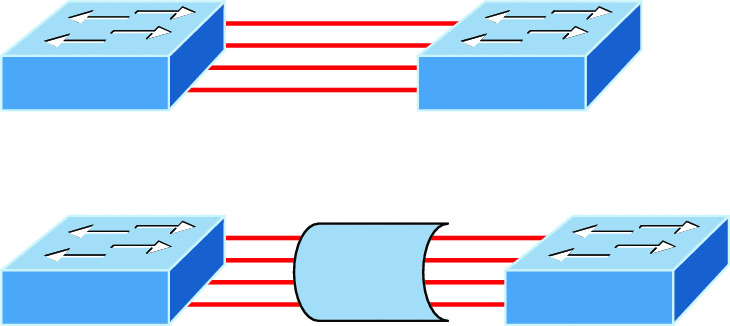
\includegraphics[width=.5\textwidth]{images/c15f020.jpg}
   \caption{Before and after port channels}
   \label{fig:etherchannel-before-after}
\end{figure}

Now as usual, there's
the Cisco version and the IEEE version of port channel negotiation
protocols to choose from -- take your pick. Cisco's version is called
Port Aggregation Protocol (PAgP), and the IEEE 802.3ad standard is
called Link Aggregation Control Protocol (LACP). Both versions work
equally well, but the way you configure each is slightly different. Keep
in mind that both PAgP and LACP are negotiation protocols and that
EtherChannel can actually be statically configured without PAgP or LACP.
Still, it's better to use one of these protocols to help with
compatibility issues as well as to manage link additions and failures
between two switches.

Cisco EtherChannel allows us to bundle up to eight ports active between
switches. The links must have the same speed, duplex setting, and VLAN
configuration -- in other words, you can't mix interface types and
configurations into the same bundle.

There are a few differences in configuring PAgP and LACP, but first,
let's go over some terms so you don't get confused:

\textbf{Port channeling} Refers to combining two to eight Fast Ethernet
or two Gigabit Ethernet ports together between two switches into one
aggregated logical link to achieve more bandwidth and resiliency.

\textbf{EtherChannel} Cisco's proprietary term for port channeling.

\textbf{PAgP} This is a Cisco proprietary port channel negotiation
protocol that aids in the automatic creation for EtherChannel links. All
links in the bundle must match the same parameters (speed, duplex, VLAN
info), and when PAgP identifies matched links, it groups the links into
an EtherChannel. This is then added to STP as a single bridge port. At
this point, PAgP's job is to send packets every 30 seconds to manage the
link for consistency, any link additions, and failures.

\textbf{LACP (802.3ad)} This has the exact same purpose as PAgP, but
it's nonproprietary so it can work between multi-vendor networks.

\texttt{channel-group} This is a command on Ethernet interfaces used to
add the specified interface to a single EtherChannel. The number
following this command is the port channel ID.

\texttt{interface\ port-channel} Here's a command that creates the
bundled interface. Ports can be added to this interface with the
\texttt{channel-group} command. Keep in mind that the interface number
must match the group number.

Now let's see if you can make some sense out of all these terms by
actually configuring something!

\subsection{Configuring and verifying port channels}

Let's use \protect\hyperlink{c15.xhtmlux5cux23figure15-21}{Figure 15.21}
for our simple example of how to configure port channels.

\begin{figure}
\centering
%\includegraphics{images/c15f021.jpg}
\caption{{\protect\hyperlink{c15.xhtmlux5cux23figureanchor15-21}{\textbf{FIGURE
15.21}} EtherChannel example}}
\end{figure}

You can enable your
\texttt{channel-group} for each channel by setting the channel mode for
each interface to either \texttt{active} or \texttt{passive} if using
LACP. When a port is configured in \texttt{passive} mode, it will
respond to the LACP packets it receives, but it won't initiate an LACP
negotiation. When a port is configured for \texttt{active} mode, the
port initiates negotiations with other ports by sending LACP packets.

Let me show you a simple example of configuring port channels and then
verifying them. First I'll go to global configuration mode and create a
port channel interface, and then I'll add this port channel to the
physical interfaces.

Remember, all parameters and configurations of the ports must be the
same, so I'll start by trunking the interfaces before I configure
EtherChannel, like this:

\begin{verbatim}
S1(config)#int range g0/1 - 2
S1(config-if-range)#switchport trunk encapsulation dot1q
S1(config-if-range)#switchport mode trunk
\end{verbatim}

All ports in your bundles must be configured the same, so I'll configure
both sides with the same trunking configuration. Now I can assign these
ports to a bundle:

\begin{verbatim}
S1(config-if-range)#channel-group 1 mode ?
  active     Enable LACP unconditionally
  auto       Enable PAgP only if a PAgP device is detected
  desirable  Enable PAgP unconditionally
  on         Enable Etherchannel only
  passive    Enable LACP only if a LACP device is detected
S1(config-if-range)#channel-group 1 mode active
S1(config-if-range)#exit
\end{verbatim}

To configure the IEEE nonproprietary LACP, I'll use the \texttt{active}
or \texttt{passive} command; if I wanted to use Cisco's PAgP, I'd use
the \texttt{auto} or \texttt{desirable} command. You can't mix and match
these on either end of the bundle, and really, it doesn't matter which
one you use in a pure Cisco environment, as long as you configure them
the same on both ends (setting the mode to \texttt{on} would be
statically configuring your EtherChannel bundle).

At this point in the configuration, I'd have to set the mode to
\texttt{active} on the S2 interfaces if I wanted the bundle to come up
with LACP because, again, all parameters must be the same on both ends
of the link. Let's configure our port channel interface, which was
created when we used the channel-group command:

\begin{verbatim}
S1(config)#int port-channel 1
S1(config-if)#switchport trunk encapsulation dot1q
S1(config-if)#switchport mode trunk
S1(config-if)#switchport trunk allowed vlan 1,2,3
\end{verbatim}

Notice that I set the same trunking method under the port channel
interface as I did the physical interfaces, as well as VLAN information
too. Nicely, all command performed under the port-channel are inherited
at the interface level, so you can just easily configure the
port-channel with all parameters.

Time to configure the interfaces, channel groups, and port channel interface on the S2 switch:

\begin{verbatim}
S2(config)#int range g0/13 - 14
S2(config-if-range)#switchport trunk encapsulation dot1q
S2(config-if-range)#switchport mode trunk
S2(config-if-range)#channel-group 1 mode active
S2(config-if-range)#exit
S2(config)#int port-channel 1
S2(config-if)#switchport trunk encapsulation dot1q
S2(config-if)#switchport mode trunk
S2(config-if)#switchport trunk allowed vlan 1,2,3
\end{verbatim}

On each switch, I configured the ports I wanted to bundle with the same
configuration, then created the port channel. After that, I added the
ports into the port channel with the \texttt{channel-group} command.

Remember, for LACP we'll use either active/active on each side of the
bundle or active/passive, but you can't use passive/passive. Same goes
for PAgP; you can use desirable/desirable or auto/desirable but not
auto/auto.

Let's verify our EtherChannel with a few commands. We'll start with the
\texttt{show\ etherchannel\ port-channel} command to see information
about a specific port channel interface:

\begin{verbatim}
S2#sh etherchannel port-channel
               Channel-group listing:
                ----------------------
 
Group: 1
----------
                Port-channels in the group:
                ---------------------------
 
Port-channel: Po1    (Primary Aggregator)
------------
 
Age of the Port-channel   = 00d:00h:46m:49s
Logical slot/port   = 2/1       Number of ports = 2
GC                  = 0x00000000      HotStandBy port = null
Port state          = Port-channel
Protocol            =   LACP
Port Security       = Disabled
 
Ports in the Port-channel:
 
Index   Load   Port     EC state        No of bits
------+------+------+------------------+-----------
  0     00     Gig0/2   Active             0
  0     00     Gig0/1   Active             0
Time since last port bundled:    00d:00h:46m:47s    Gig0/1
S2#
\end{verbatim}

Notice that we have one group and that we're running the IEEE LACP
version of port channeling. We're in \texttt{Active} mode, and that
\texttt{Port-channel:\ Po1} interface has two physical interfaces. The
heading \texttt{Load} is not the load over the interfaces, it's a
hexadecimal value that decides which interface will be chosen to specify
the flow of traffic.

The \texttt{show\ etherchannel\ summary} command displays one line of
information per port channel:

\begin{verbatim}
S2#sh etherchannel summary
Flags:  D - down        P - in port-channel
        I - stand-alone s - suspended
        H - Hot-standby (LACP only)
        R - Layer3      S - Layer2
        U - in use      f - failed to allocate aggregator
        u - unsuitable for bundling
        w - waiting to be aggregated
        d - default port
 
Number of channel-groups in use: 1
Number of aggregators:           1
 
Group  Port-channel  Protocol    Ports
------+-------------+-----------+----------------------------------------------
 
1      Po1(SU)           LACP   Gig0/1(P) Gig0/2(P)
\end{verbatim}

This command shows that we have one group, that we're running LACP, and
Gig0/1 and Gig0/2 or (P), which means these ports are
\texttt{in\ port-channel} mode. This command isn't really all that
helpful unless you have multiple channel groups, but it does tell us our
group is working well!

\subsubsection{Layer~3 EtherChannel}

One last item to discuss before we finish this chapter and that is layer
3 EtherChannel. You'd use layer~3 EtherChannel when connecting a switch
to multiple ports on a router, for example. It's important to understand
that you wouldn't put IP addresses under the physical interfaces
of the router, instead you'd actually add the IP address of the bundle
under the logical port-channel interface.

Here is an example on how to create the logical port channel 1 and
assign 20.2.2.2 as its IP address:

\begin{verbatim}
Router#config t
Router(config)#int port-channel 1
Router(config-if)#ip address 20.2.2.2 255.255.255.0
\end{verbatim}

Now we need to add the physical ports into port channel 1:

\begin{verbatim}
Router(config-if)#int range g0/0-1
Router(config-if-range)#channel-group 1
GigabitEthernet0/0 added as member-1 to port-channel1
GigabitEthernet0/1 added as member-2 to port-channel1
\end{verbatim}

Now let's take a look at the running-config. Notice there are no IP
addresses under the physical interface of the router:

\begin{verbatim}
!
interface Port-channel1
 ip address 20.2.2.2 255.255.255.0
 load-interval 30
!
 interface GigabitEthernet0/0
 no ip address
 load-interval 30
 duplex auto
 speed auto
 channel-group 1
!
 interface GigabitEthernet0/1
 no ip address
 load-interval 30
 duplex auto
 speed auto
 channel-group 1
\end{verbatim}

\section{Summary}

This chapter was all about switching technologies, with a particular focus on the Spanning-Tree Protocol (STP) and its evolution to newer
versions like RSTP and then Cisco's PVST+.

You learned about the problems that can occur if you have multiple links between bridges (switches) and the solutions attained with STP.

I also talked about and demonstrated issues that can occur if you have multiple links between bridges (switches), plus how to solve these
problems by using the Spanning-Tree Protocol (STP).

I covered a detailed configuration of Cisco's Catalyst switches, including verifying the configuration, setting the Cisco STP extensions,
and changing the root bridge by setting a bridge priority.

Finally, we discussed, configured, and verified the EtherChannel technology that helps us bundle multiple links between switches.




\section{Exam essentials}

\textbf{Understand the main purpose of the Spanning Tree Protocol in a
switched LAN.} The main purpose of STP is to prevent switching loops in
a network with redundant switched paths.

\textbf{Remember the states of STP.} The purpose of the blocking state
is to prevent the use of looped paths. A port in listening state
prepares to forward data frames without populating the MAC address
table. A port in learning state populates the MAC address table but
doesn't forward data frames. A port in forwarding state sends and
receives all data frames on the bridged port. Also, a port in the
disabled state is virtually nonoperational.

\textbf{Remember the command}\texttt{show\ spanning-tree}. You must be
familiar with the command \texttt{show\ spanning-tree} and how to
determine the root bridge of each VLAN. Also, you can use the
\texttt{show\ spanning-tree\ summary} command to help you get a quick
glimpse of your STP network and root bridges.

\textbf{Understand what PortFast and BPDU Guard provide.} PortFast
allows a port to transition to the forwarding state immediately upon a
connection. Because you don't want other switches connecting to this
port, BPDU Guard will shut down a PortFast port if it receives a BPDU.

\textbf{Understand what EtherChannel is and how to configure it.}
EtherChannel allows you to bundle links to get more bandwidth, instead
of allowing STP to shut down redundant ports. You can configure Cisco's
PAgP or the IEEE version, LACP, by creating a port channel interface and
assigning the port channel group number to the interfaces you are
bundling.

\section{Written lab}

You can find the answers to this lab in Appendix A, ``Answers to Written
Labs.''

Write the answers to the following questions:

\begin{enumerate}
\tightlist
\item
  Which of the following is Cisco proprietary: LACP or PAgP?
\item
  What command will show you the STP root bridge for a VLAN?
\item
  What standard is
  RSTP PVST+ based on?
\item
  Which protocol is used in a layer~2 network to maintain a loop-free
  network?
\item
  Which proprietary Cisco STP extension would put a switch port into
  error disabled mode if a BPDU is received on this port?
\item
  You want to configure a switch port to not transition through the STP
  port states but to go immediately to forwarding mode. What command
  will you use on a per-port basis?
\item
  What command will you use to see information about a specific port
  channel interface?
\item
  What command can you use to set a switch so that it will be the root
  bridge for VLAN 3 over any other switch?
\item
  You need to find the VLANs for which your switch is the root bridge.
  What two commands can you use?
\item
  What are the two modes you can set with LACP?
\end{enumerate}

\section{Hands-on labs}

In this section, you will configure and verify STP, as well as configure
PortFast and BPDU Guard, and finally, bundle links together with
EtherChannel.

Note that the labs in this chapter were written to be used with real
equipment using 2960 switches. However, you can use the free LammleSim
IOS version simulator or Cisco's Packet Tracer to run through these
labs.

The labs in this chapter are as follows:

\begin{enumerate}
\tightlist
\item
  Lab 15.1: Verifying STP and Finding Your Root Bridge
\item
  Lab 15.2: Configuring and Verifying Your Root Bridge
\item
  Lab 15.3: Configuring PortFast and BPDU Guard
\item
  Lab 15.4: Configuring and Verifying EtherChannel
\item
  We'll use the following illustration for all four labs:
\end{enumerate}

\begin{figure}
\centering
%\includegraphics{images/c15f022.jpg}
\caption{}
\end{figure}

\subsubsection[Hands-on Lab 15.1: Verifying STP and Finding Your Root
Bridge]{\texorpdfstring{\protect\hypertarget{c15.xhtmlux5cux23c15-sec-25}{}{}Hands-on
Lab 15.1: Verifying STP and Finding Your Root
Bridge}{Hands-on Lab 15.1: Verifying STP and Finding Your Root Bridge}}

This lab will assume that you have added VLANs 2 and 3 to each of your
switches and all of your links are trunked.

\begin{enumerate}
\item
  From one of your switches, use the
  \texttt{show\ spanning-tree\ vlan\ 2} command. Verify the output.

\begin{verbatim}
S3#sh spanning-tree vlan 2
VLAN0002
  Spanning tree enabled protocol ieee
  Root ID    Priority    32770
             Address     0001.C9A5.8748
             Cost        19
             Port        1(FastEthernet0/1)
             Hello Time  2 sec  Max Age 20 sec  Forward Delay 15 sec
 
  Bridge ID  Priority    32770  (priority 32768 sys-id-ext 2)
             Address     0004.9A04.ED97
             Hello Time  2 sec  Max Age 20 sec  Forward Delay 15 sec
             Aging Time  20
\end{verbatim}

\begin{verbatim}
Interface        Role Sts Cost      Prio.Nbr Type
---------------- ---- --- --------- -------- --------------------------------
Fa0/1            Root FWD 19        128.1    P2p
Fa0/2            Desg FWD 19        128.2    P2p
Gi1/1            Altn BLK 4         128.25   P2p
Gi1/2            Altn BLK 4         128.26   P2p
\end{verbatim}

  Notice that S3 is not the root bridge, so to find your root bridge,
  just follow the root port and see what bridge is connected to that
  port. Port Fa0/1 is the root port with a cost of 19, which means the
  switch that is off the Fa0/1 port is the root port connecting to the
  root bridge because it is a cost of 19, meaning one Fast Ethernet link
  away.
\item
  Find the bridge that is off of Fa0/1, which will be our root.

\begin{verbatim}
S3#sh cdp neighbors
Capability Codes: R - Router, T - Trans Bridge, B - Source Route Bridge
                  S - Switch, H - Host, I - IGMP, r - Repeater, P - Phone
Device ID    Local Intrfce   Holdtme    Capability   Platform    Port ID
S1           Fas 0/1          158            S       2960        Fas 0/1
S2           Gig 1/1          151            S       2960        Gig 1/1
S2           Gig 1/2          151            S       2960        Gig 1/2
S3#
\end{verbatim}

  Notice that S1 is connected to the local interface Fa0/1, so let's go
  to S1 and verify our root bridge.
\item
  Verify the root bridge for each of the three VLANs. From S1, use the
  \texttt{show\ spanning-tree\ summary} command.

\begin{verbatim}
S1#sh spanning-tree summary
Switch is in pvst mode
Root bridge for: default VLAN0002 VLAN0003
Extended system ID           is enabled
Portfast Default             is disabled
PortFast BPDU Guard Default  is disabled
Portfast BPDU Filter Default is disabled
Loopguard Default            is disabled
EtherChannel misconfig guard is disabled
UplinkFast                   is disabled
BackboneFast                 is disabled
Configured Pathcost method used is short
 
Name                   Blocking Listening Learning Forwarding STP Active
---------------------- -------- --------- -------- ---------- ----------
VLAN0001                     0         0        0          2          2
VLAN0002                     0         0        0          2          2
VLAN0003                     0         0        0          2          2
 
---------------------- -------- --------- -------- ---------- ----------
3 vlans                      0         0        0          6          6
 
S1#
\end{verbatim}

  Notice that S1 is the root bridge for all three VLANs.
\item
  Make note of all your root bridges, for all three VLANs, if you have
  more than one root bridge.
\end{enumerate}

\subsubsection[Hands-on Lab 15.2: Configuring and Verifying Your Root
Bridge]{\texorpdfstring{\protect\hypertarget{c15.xhtmlux5cux23c15-sec-26}{}{}Hands-on
Lab 15.2: Configuring and Verifying Your Root
Bridge}{Hands-on Lab 15.2: Configuring and Verifying Your Root Bridge}}

This lab will assume you have performed Lab 1 and now know who your root
bridge is for each VLAN.

\begin{enumerate}
\item
  Go to one of your
  non-root bridges and verify the bridge ID with the
  \texttt{show\ spanning-tree\ vlan} command.

\begin{verbatim}
S3#sh spanning-tree vlan 1
VLAN0001
  Spanning tree enabled protocol ieee
  Root ID    Priority    32769
             Address     0001.C9A5.8748
             Cost        19
             Port        1(FastEthernet0/1)
             Hello Time  2 sec  Max Age 20 sec  Forward Delay 15 sec
 
  Bridge ID  Priority    32769  (priority 32768 sys-id-ext 1)
             Address     0004.9A04.ED97
             Hello Time  2 sec  Max Age 20 sec  Forward Delay 15 sec
             Aging Time  20
 
Interface        Role Sts Cost      Prio.Nbr Type
---------------- ---- --- --------- -------- --------------------------------
Fa0/1            Root FWD 19        128.1    P2p
Fa0/2            Desg FWD 19        128.2    P2p
Gi1/1            Altn BLK 4         128.25   P2p
Gi1/2            Altn BLK 4         128.26   P2p
\end{verbatim}

  Notice that this bridge is not the root bridge for VLAN 1 and the root
  port is Fa0/1 with a cost of 19, which means the root bridge is
  directly connected one Fast Ethernet link away.
\item
  Make one of your non-root bridges the root bridge for VLAN 1. Use
  priority 16,384, which is lower than the 32,768 of the current root.

\begin{verbatim}
S3(config)#spanning-tree vlan 1 priority ?
  <0-61440>  bridge priority in increments of 4096
S3(config)#spanning-tree vlan 1 priority 16384
\end{verbatim}
\item
  Verify the root bridge for VLAN 1.

\begin{verbatim}
S3#sh spanning-tree vlan 1
VLAN0001
  Spanning tree enabled protocol ieee
  Root ID    Priority    16385
             Address     0004.9A04.ED97
             This bridge is the root
             Hello Time  2 sec  Max Age 20 sec  Forward Delay 15 sec
 
  Bridge ID  Priority    16385  (priority 16384 sys-id-ext 1)
             Address     0004.9A04.ED97
             Hello Time  2 sec  Max Age 20 sec  Forward Delay 15 sec
             Aging Time  20
 
Interface        Role Sts Cost      Prio.Nbr Type
---------------- ---- --- --------- -------- --------------------------------
Fa0/1            Desg FWD 19        128.1    P2p
Fa0/2            Desg FWD 19        128.2    P2p
Gi1/1            Desg FWD 4         128.25   P2p
Gi1/2            Desg FWD 4         128.26   P2p
\end{verbatim}
\end{enumerate}

Notice that this bridge is indeed the root and all ports are in Desg FWD
mode.

\subsubsection[Hands-on Lab 15.3: Configuring PortFast and BPDU
Guard]{\texorpdfstring{\protect\hypertarget{c15.xhtmlux5cux23c15-sec-27}{}{}Hands-on
Lab 15.3: Configuring PortFast and BPDU
Guard}{Hands-on Lab 15.3: Configuring PortFast and BPDU Guard}}

This lab will have you configure ports on switches S3 and S2 to allow
the PC and server to automatically go into forward mode when they
connect into the port.

\begin{enumerate}
\item
  Connect to your switch that has a host connected and enable PortFast
  for the interface.

\begin{verbatim}
S3#config t
S3(config)#int fa0/2
S3(config-if)#spanning-tree portfast
%Warning: portfast should only be enabled on ports connected to a single
host. Connecting hubs, concentrators, switches, bridges, etc... to this
interface  when portfast is enabled, can cause temporary bridging loops.
Use with CAUTION
\end{verbatim}

\begin{verbatim}
 
%Portfast has been configured on FastEthernet0/2 but will only
have effect when the interface is in a non-trunking mode.
\end{verbatim}
\item
  Verify that the switch port will be shut down if another switch
  Ethernet cable plugs into this port.

\begin{verbatim}
S3(config-if)#spanning-tree bpduguard enable
\end{verbatim}
\item
  Verify your configuration with the \texttt{show\ running-config}
  command.

\begin{verbatim}
!
interface FastEthernet0/2
 switchport mode trunk
 spanning-tree portfast
 spanning-tree bpduguard enable
!
\end{verbatim}
\end{enumerate}

\subsubsection[Hands-on Lab 15.4: Configuring and Verifying
EtherChannel]{\texorpdfstring{\protect\hypertarget{c15.xhtmlux5cux23c15-sec-28}{}{}Hands-on
Lab 15.4: Configuring and Verifying
EtherChannel}{Hands-on Lab 15.4: Configuring and Verifying EtherChannel}}

This lab will have you configure the Cisco EtherChannel PAgP version on
the switches used in this lab. Because I have preconfigured the
switches, I have set up the trunks on all inter-switch ports. We'll use
the Gigabit Ethernet ports between switches S3 and S2.

\begin{enumerate}
\item
  Configure the S3 switch with EtherChannel by creating a port channel
  interface.

\begin{verbatim}
S3#config t
S3(config)#inter port-channel 1
\end{verbatim}
\item
  Configure the ports to be in the bundle with the
  \texttt{channel-group} command.

\begin{verbatim}
S3(config-if)#int range g1/1 - 2
S3(config-if-range)#channel-group 1 mode ?
  active     Enable LACP unconditionally
  auto       Enable PAgP only if a PAgP device is detected
  desirable  Enable PAgP unconditionally
  on         Enable Etherchannel only
  passive    Enable LACP only if a LACP device is detected
S3(config-if-range)#channel-group 1 mode desirable
\end{verbatim}

  I chose the PAgP desirable mode for the S3 switch.
\item
  Configure the S2 switch with EtherChannel, using the same parameters
  as S3.

\begin{verbatim}
S2#config t
S2(config)#interface port-channel 1
S2(config-if)#int rang g1/1 - 2
S2(config-if-range)#channel-group 1 mode desirable
%LINK-5-CHANGED: Interface Port-channel 1, changed state to up
\end{verbatim}

\begin{verbatim}
 %LINEPROTO-5-UPDOWN: Line protocol on Interface Port-channel 1, changed state to up
\end{verbatim}

  Pretty simple, really. Just a couple of commands.
\item
  Verify with the \texttt{show\ etherchannel\ port-channel} command.

\begin{verbatim}
S3#sh etherchannel port-channel
                Channel-group listing:
                ----------------------

Group: 1
----------
                Port-channels in the group:
                ---------------------------
 
Port-channel: Po1
------------
 
Age of the Port-channel   = 00d:00h:06m:43s
Logical slot/port   = 2/1       Number of ports = 2
GC                  = 0x00000000      HotStandBy port = null
Port state          = Port-channel
Protocol            =   PAGP
Port Security       = Disabled
 
Ports in the Port-channel:
 
Index   Load   Port     EC state        No of bits
------+------+------+------------------+-----------
  0     00     Gig1/1   Desirable-Sl       0
  0     00     Gig1/2   Desirable-Sl       0
Time since last port bundled:    00d:00h:01m:30s    Gig1/2
\end{verbatim}
\item
  Verify with the \texttt{show\ etherchannel\ summary} command.

\begin{verbatim}
S3#sh etherchannel summary
Flags:  D - down        P - in port-channel
        I - stand-alone s - suspended
        H - Hot-standby (LACP only)
        R - Layer3      S - Layer2
        U - in use      f - failed to allocate aggregator
        u - unsuitable for bundling
        w - waiting to be aggregated
        d - default port
 
Number of channel-groups in use: 1
Number of aggregators:           1
 
Group  Port-channel  Protocol    Ports
------+-------------+-----------+----------------------------------
 
1      Po1(SU)           PAgP   Gig1/1(P) Gig1/2(P)
S3#
\end{verbatim}
\end{enumerate}

\section{Review questions}

\begin{center}\rule{0.5\linewidth}{0.5pt}\end{center}

%\includegraphics{images/note.png}
The following questions are designed to
test your understanding of this chapter's material. For more information
on how to get additional questions, please see
\texttt{www.lammle.com/ccna}.

\begin{center}\rule{0.5\linewidth}{0.5pt}\end{center}

You can find the answers to these questions in Appendix B, ``Answers to
Review Questions.''

\begin{enumerate}
\item
  You receive the following output from a switch:

\begin{verbatim}
S2#sh spanning-tree
VLAN0001
  Spanning tree enabled protocol rstp
  Root ID    Priority    32769
             Address     0001.42A7.A603
             Cost        4
             Port        26(GigabitEthernet1/2)
             Hello Time  2 sec  Max Age 20 sec  Forward Delay 15 sec
[output cut]
\end{verbatim}

  Which are true regarding this switch? (Choose two.)

  \begin{enumerate}
  \tightlist
  \item
    The switch is a root bridge.
  \item
    The switch is a non-root bridge.
  \item
    The root bridge is four switches away.
  \item
    The switch is running 802.1w.
  \item
    The switch is running STP PVST+.
  \end{enumerate}
\item
  You have configured your switches with the
  \texttt{spanning-tree\ vlan\ x\ root\ primary} and
  \texttt{spanning-tree\ vlan\ x\ root\ secondary}commands. Which of the
  following tertiary switch will take over if both switches fail?

  \begin{enumerate}
  \tightlist
  \item
    A switch with priority 4096
  \item
    A switch with priority 8192
  \item
    A switch with priority 12288
  \item
    A switch with priority 20480
  \end{enumerate}
\item
  Which of the following would you use to find the VLANs for which your
  switch is the root bridge? (Choose two.)

  \begin{enumerate}
  \tightlist
  \item
    \texttt{show\ spanning-tree}
  \item
    \texttt{show\ root\ all}
  \item
    \texttt{show\ spanning-tree\ port\ root\ VLAN}
  \item
    \texttt{show\ spanning-tree\ summary}
  \end{enumerate}
\item
  You want to run the
  new 802.1w on your switches. Which of the following would enable this
  protocol?

  \begin{enumerate}
  \tightlist
  \item
    \texttt{Switch(config)\#spanning-tree\ mode\ rapid-pvst}
  \item
    \texttt{Switch\#spanning-tree\ mode\ rapid-pvst}
  \item
    \texttt{Switch(config)\#spanning-tree\ mode\ 802.1w}
  \item
    \texttt{Switch\#spanning-tree\ mode\ 802.1w}
  \end{enumerate}
\item
  Which of the following is a layer~2 protocol used to maintain a
  loop-free network?

  \begin{enumerate}
  \tightlist
  \item
    VTP
  \item
    STP
  \item
    RIP
  \item
    CDP
  \end{enumerate}
\item
  Which statement describes a spanning-tree network that has converged?

  \begin{enumerate}
  \tightlist
  \item
    All switch and bridge ports are in the forwarding state.
  \item
    All switch and bridge ports are assigned as either root or
    designated ports.
  \item
    All switch and bridge ports are in either the forwarding or blocking
    state.
  \item
    All switch and bridge ports are either blocking or looping.
  \end{enumerate}
\item
  Which of the following modes enable LACP EtherChannel? (Choose two.)

  \begin{enumerate}
  \tightlist
  \item
    On
  \item
    Prevent
  \item
    Passive
  \item
    Auto
  \item
    Active
  \item
    Desirable
  \end{enumerate}
\item
  Which of the following are true regarding RSTP? (Choose three.)

  \begin{enumerate}
  \tightlist
  \item
    RSTP speeds the recalculation of the spanning tree when the layer~2
    network topology changes.
  \item
    RSTP is an IEEE standard that redefines STP port roles, states, and
    BPDUs.
  \item
    RSTP is extremely proactive and very quick, and therefore it
    absolutely needs the 802.1 delay timers.
  \item
    RSTP (802.1w) supersedes 802.1d while remaining proprietary.
  \item
    All of the 802.1d terminology and most parameters have been changed.
  \item
    802.1w is capable of reverting to 802.1d to interoperate with
    traditional switches on a per-port basis.
  \end{enumerate}
\item
  What does BPDU Guard perform?

  \begin{enumerate}
  \tightlist
  \item
    Makes sure the port is receiving BPDUs from the correct upstream
    switch.
  \item
    Makes sure the port is not receiving BPDUs from the upstream switch,
    only the root.
  \item
    If a BPDU is
    received on a BPDU Guard port, PortFast is used to shut down the
    port.
  \item
    Shuts down a port if a BPDU is seen on that port.
  \end{enumerate}
\item
  How many bits is the \texttt{sys-id-ext} field in a BPDU?

  \begin{enumerate}
  \tightlist
  \item
    4
  \item
    8
  \item
    12
  \item
    16
  \end{enumerate}
\item
  There are four connections between two switches running RSTP PVST+ and
  you want to figure out how to achieve higher bandwidth without
  sacrificing the resiliency that RSTP provides. What can you configure
  between these two switches to achieve higher bandwidth than the
  default configuration is already providing?

  \begin{enumerate}
  \tightlist
  \item
    Set PortFast and BPDU Guard, which provides faster convergence.
  \item
    Configure unequal cost load balancing with RSTP PVST+.
  \item
    Place all four links into the same EtherChannel bundle.
  \item
    Configure PPP and use multilink.
  \end{enumerate}
\item
  In which circumstance are multiple copies of the same unicast frame
  likely to be transmitted in a switched LAN?

  \begin{enumerate}
  \tightlist
  \item
    During high-traffic periods
  \item
    After broken links are reestablished
  \item
    When upper-layer protocols require high reliability
  \item
    In an improperly implemented redundant topology
  \end{enumerate}
\item
  You want to configure LACP. Which do you need to make sure are
  configured exactly the same on all switch interfaces you are using?
  (Choose three.)

  \begin{enumerate}
  \tightlist
  \item
    Virtual MAC address
  \item
    Port speeds
  \item
    Duplex
  \item
    PortFast enabled
  \item
    VLAN information
  \end{enumerate}
\item
  Which of the following modes enable PAgP EtherChannel? (Choose two.)

  \begin{enumerate}
  \tightlist
  \item
    On
  \item
    Prevent
  \item
    Passive
  \item
    Auto
  \item
    Active
  \item
    Desirable
  \end{enumerate}
\item
  For this question,
  refer to the following illustration. SB's RP to the root bridge has
  failed.

  \begin{figure}
  \centering
  %\includegraphics{images/c15f023.jpg}
  \caption{}
  \end{figure}

  What is the new cost for SB to make a single path to the root bridge?

  \begin{enumerate}
  \tightlist
  \item
    4
  \item
    8
  \item
    23
  \item
    12
  \end{enumerate}
\item
  Which of the following would put switch interfaces into EtherChannel
  port number 1, using LACP? (Choose two.)

  \begin{enumerate}
  \tightlist
  \item
    \texttt{Switch(config)\#interface\ port-channel\ 1}
  \item
    \texttt{Switch(config)\#channel-group\ 1\ mode\ active}
  \item
    \texttt{Switch\#interface\ port-channel\ 1}
  \item
    \texttt{Switch(config-if)\#channel-group\ 1\ mode\ active}
  \end{enumerate}
\item
  Which two commands would guarantee your switch to be the root bridge
  for VLAN 30? (Choose two.)

  \begin{enumerate}
  \tightlist
  \item
    \texttt{spanning-tree\ vlan\ 30\ priority\ 0}
  \item
    \texttt{spanning-tree\ vlan\ 30\ priority\ 16384}
  \item
    \texttt{spanning-tree\ vlan\ 30\ root\ guarantee}
  \item
    \texttt{spanning-tree\ vlan\ 30\ root\ primary}
  \end{enumerate}
\item
  Why does Cisco use its proprietary extension of PVST+ with STP and
  RSTP?

  \begin{enumerate}
  \tightlist
  \item
    Root bridge placement enables faster convergence as well as optimal
    path determination.
  \item
    Non-root bridge placement clearly enables faster convergence as well
    as optimal path determination.
  \item
    PVST+ allows for
    faster discarding of non-IP frames.
  \item
    PVST+ is actually an IEEE standard called 802.1w.
  \end{enumerate}
\item
  Which are states in 802.1d? (Choose all that apply.)

  \begin{enumerate}
  \tightlist
  \item
    Blocking
  \item
    Discarding
  \item
    Listening
  \item
    Learning
  \item
    Forwarding
  \item
    Alternate
  \end{enumerate}
\item
  Which of the following are roles in STP? (Choose all that apply.)

  \begin{enumerate}
  \tightlist
  \item
    Blocking
  \item
    Discarding
  \item
    Root
  \item
    Non-designated
  \item
    Forwarding
  \item
    Designated
  \end{enumerate}
\end{enumerate}

